\documentclass{article}
\usepackage[
  a4paper,
  left=2cm, right=2cm,
  top=2cm, bottom=2cm
]{geometry}
\usepackage{graphicx} % Required for inserting images
\usepackage{amsmath}       % Équations avancées
\usepackage{amssymb}       % Symboles mathématiques
\usepackage{graphicx}      % Inclusion de figures
\usepackage{siunitx}       % Unités SI
\usepackage{setspace}
\singlespacing
\usepackage{multirow}
\usepackage{booktabs}      % Tableaux professionnels
\usepackage[table]{xcolor}
\usepackage{hyperref}      % Références cliquables
\usepackage[most]{tcolorbox}
\usepackage{bm}
\usepackage{float}

\usepackage[framemethod=TikZ]{mdframed}
\usepackage{pgfplots}   
\usepackage{caption}   

\usepackage{enumitem}
\usepackage{titlesec}
\usepackage{wasysym}
\usepackage{tikz}
\usetikzlibrary{positioning,arrows.meta,shapes.geometric,decorations.pathreplacing,calc,3d,positioning,patterns} % pour "below=of ..." et "-Stealth"
\usepackage{tikz-3dplot}

\usepackage{algorithm}
\usepackage{algorithmic}

\usepackage{listings}
\usetikzlibrary{shapes,arrows,positioning,calc}

\usepackage{fancyvrb}
\usepackage{fvextra}
\usepackage{pifont}
\usepackage{colortbl}

\newcommand{\codeTight}{\fontsize{8pt}{9pt}\selectfont} 

\captionsetup{font=footnotesize,labelfont=bf,textfont=it,skip=0pt}

% Commandes personnalisées
\newcommand{\cmark}{\textcolor{successgreen}{\ding{51}}}
\newcommand{\xmark}{\textcolor{errorred}{\ding{55}}}
\newcommand{\wmark}{\textcolor{warningorange}{\ding{45}}}


% --- Espaces autour des flottants (tables, figures) ---
\setlength{\textfloatsep}{8pt plus 2pt minus 2pt}
\setlength{\floatsep}{8pt plus 2pt minus 2pt}
\setlength{\intextsep}{8pt plus 2pt minus 2pt}
\setlength{\abovecaptionskip}{4pt}
\setlength{\belowcaptionskip}{0pt}

% --- Listes pour tout le document ---
\setlist[itemize]{itemsep=0pt, topsep=2pt, parsep=0pt, partopsep=0pt}
\setlist[enumerate]{itemsep=0pt, topsep=2pt, parsep=0pt, partopsep=0pt}

% --- Espaces autour des titres ---
\titlespacing*{\section}
  {0pt}{2ex plus 1ex minus .2ex}{1ex plus .5ex minus .2ex}
\titlespacing*{\subsection}
  {0pt}{1.5ex plus .5ex minus .2ex}{0.7ex plus .3ex minus .1ex}

% --- Espaces autour des formules affichées ---
\setlength{\abovedisplayskip}{6pt}
\setlength{\belowdisplayskip}{6pt}
\setlength{\abovedisplayshortskip}{4pt}
\setlength{\belowdisplayshortskip}{4pt}

\definecolor{misty}{rgb}{1.0,0.89,0.88}
\definecolor{MyBlue}{rgb}{0.8,1.0,1.0}
\definecolor{Carnelian}{rgb}{0.7,0.11,0.11}
\definecolor{MyGreen}{rgb}{0.0,0.5,0.0}
\definecolor{MyGreen2}{rgb}{0.0,0.42,0.24}
\definecolor{corrigecolor}{RGB}{180,100,200}
\definecolor{methode1color}{RGB}{220,80,60}
\definecolor{methode2color}{RGB}{80,180,80}
\definecolor{lightblue}{RGB}{220,235,255}
\definecolor{successgreen}{RGB}{39,174,96}
\definecolor{warningorange}{RGB}{243,156,18}
\definecolor{errorred}{RGB}{231,76,60}
\definecolor{infoblue}{RGB}{52,152,219}
\definecolor{darkblue}{RGB}{44,62,80}
\definecolor{lightgray}{RGB}{245,245,245}
\definecolor{purple}{RGB}{142,68,173}
\definecolor{lightgray}{RGB}{245,245,245}
\definecolor{okgreen}{RGB}{39,174,96}
\definecolor{warnorange}{RGB}{230,126,34}

% Couleurs personnalisées
\definecolor{aircolor}{RGB}{200, 220, 255}
\definecolor{tungcolor}{RGB}{255, 220, 200}
\definecolor{ratiocolor}{RGB}{220, 255, 220}

% Couleurs personnalisées
\definecolor{aircolor}{RGB}{220, 220, 220}
\definecolor{tungcolor}{RGB}{255, 220, 200}
\definecolor{pmmacolor}{RGB}{200, 255, 200}
\definecolor{ratiocolor}{RGB}{200, 220, 255}


% Définition des couleurs
\definecolor{tungsten}{RGB}{100,100,120}
\definecolor{wpetg}{RGB}{80,80,100}
\definecolor{water}{RGB}{100,180,255}
\definecolor{waterlight}{RGB}{150,200,255}
\definecolor{source}{RGB}{255,200,0}
\definecolor{cone1}{RGB}{255,100,100}
\definecolor{cone2}{RGB}{100,100,255}

\definecolor{source}{RGB}{255,200,0}
\definecolor{cone20}{RGB}{100,150,255}
\definecolor{cone60}{RGB}{255,150,100}
\definecolor{water}{RGB}{100,180,255}


% Configuration des couleurs
\definecolor{typeA}{RGB}{231,76,60}
\definecolor{typeB}{RGB}{241,196,15}
\definecolor{typeC}{RGB}{230,126,34}
\definecolor{typeD0}{RGB}{155,89,182}
\definecolor{typeD1}{RGB}{52,152,219}
\definecolor{typeD2}{RGB}{26,188,156}
\definecolor{typeD3}{RGB}{46,204,113}
\definecolor{typeD4}{RGB}{149,165,166}

\definecolor{methode1}{RGB}{70,130,180}
\definecolor{methode1bis}{RGB}{60,179,113}
\definecolor{methode2}{RGB}{255,140,0}
\definecolor{theoriecolor}{RGB}{0,100,180}

% Couleurs
\definecolor{darkblue}{RGB}{0,51,102}
\definecolor{lightblue}{RGB}{230,240,250}
\definecolor{lightgreen}{RGB}{230,250,230}
\definecolor{lightorange}{RGB}{255,240,220}
\definecolor{lightred}{RGB}{255,230,230}
\definecolor{method1}{RGB}{70,130,180}
\definecolor{method1bis}{RGB}{60,179,113}
\definecolor{method2}{RGB}{255,140,0}

% Couleurs pour la figure
\definecolor{filtercolor}{RGB}{128,128,153}
\definecolor{containercolor}{RGB}{102,102,115}
\definecolor{watercolor}{RGB}{51,153,255}
\definecolor{prefiltercolor}{RGB}{0,255,0}
\definecolor{postfiltercolor}{RGB}{255,255,0}
\definecolor{precontainercolor}{RGB}{255,128,0}
\definecolor{postcontainercolor}{RGB}{128,0,128}
\definecolor{prewatercolor}{RGB}{0,255,255}
\definecolor{postwatercolor}{RGB}{255,0,255}


% Couleurs
\definecolor{sourcecolor}{RGB}{255, 50, 50}
\definecolor{conecolor}{RGB}{255, 150, 150}
\definecolor{pmmacolor}{RGB}{255, 180, 100}
\definecolor{watercolor}{RGB}{100, 150, 255}
\definecolor{usefulcolor}{RGB}{100, 200, 100}
\definecolor{lostcolor}{RGB}{200, 200, 200}
\definecolor{solidanglecolor}{RGB}{100, 200, 100}

% Couleurs personnalisées
\definecolor{sourcecolor}{RGB}{255,100,0}
\definecolor{matrixcolor}{RGB}{255,220,100}
\definecolor{upstreamcolor}{RGB}{100,100,255}
\definecolor{downstreamcolor}{RGB}{255,100,100}
\definecolor{watercolor}{RGB}{100,180,255}
\definecolor{conecolor}{RGB}{255,200,100}
\definecolor{aircolor}{RGB}{240,248,255}
\definecolor{warningcolor}{RGB}{255,150,0}
\definecolor{energie40}{RGB}{255,100,100}
\definecolor{energie122}{RGB}{255,150,50}
\definecolor{energie344}{RGB}{255,200,50}
\definecolor{energie779}{RGB}{150,200,50}
\definecolor{energie964}{RGB}{50,200,100}
\definecolor{energie1408}{RGB}{50,150,200}

% Couleurs personnalisées
\definecolor{airblue}{RGB}{135,206,250}
\definecolor{sourcemagenta}{RGB}{255,0,255}
\definecolor{conecolor}{RGB}{255,200,0}
\definecolor{kermacolor}{RGB}{0,255,255}
\definecolor{upstreamblue}{RGB}{0,0,255}
\definecolor{downstreamred}{RGB}{255,0,0}
\definecolor{slabcolor}{RGB}{255,255,0}
\definecolor{plaquecolor}{RGB}{100,200,100}
\definecolor{cone60color}{RGB}{100,200,100}
\definecolor{cone7color}{RGB}{255,150,150}

% Couleurs personnalisées
\definecolor{precontainer}{RGB}{255,165,0}
\definecolor{postcontainer}{RGB}{0,139,139}
\definecolor{backscatter}{RGB}{148,0,211}

% Définition des couleurs
\definecolor{pmma}{RGB}{255, 180, 120}
\definecolor{water}{RGB}{100, 180, 255}
\definecolor{tungsten}{RGB}{80, 80, 80}
\definecolor{container}{RGB}{180, 180, 180}
\definecolor{preplane}{RGB}{255, 150, 50}
\definecolor{postplane}{RGB}{160, 100, 220}
\definecolor{wpetg}{RGB}{140, 140, 160}

% Définition des couleurs
\definecolor{headercolor}{RGB}{70, 130, 180}
\definecolor{successcolor}{RGB}{34, 139, 34}
\definecolor{photocolor}{RGB}{255, 200, 200}
\definecolor{comptoncolor}{RGB}{200, 200, 255}
\definecolor{paircolor}{RGB}{200, 255, 200}

% Couleurs personnalisées
\definecolor{sourcecolor}{RGB}{255,100,100}
\definecolor{slabcolor}{RGB}{255,230,100}
\definecolor{upstreamcolor}{RGB}{100,150,255}
\definecolor{downstreamcolor}{RGB}{255,100,100}
\definecolor{kermacolor}{RGB}{100,255,255}
\definecolor{aircolor}{RGB}{220,240,255}
\definecolor{conecolor}{RGB}{255,200,150}
\definecolor{worldcolor}{RGB}{240,240,240}
\definecolor{envelopecolor}{RGB}{200,220,255}

\definecolor{transmitcolor}{RGB}{46,204,113}
\definecolor{absorbcolor}{RGB}{231,76,60}
\definecolor{scattercolor}{RGB}{241,196,15}
\definecolor{oldcolor}{RGB}{180,180,180}

% Couleurs personnalisées
\definecolor{aircolor}{RGB}{200,230,255}
\definecolor{watercolor}{RGB}{100,150,255}
\definecolor{sourcecolor}{RGB}{255,80,80}
\definecolor{detectorcolor}{RGB}{100,200,100}
\definecolor{conecolor}{RGB}{255,180,100}
\definecolor{cone7color}{RGB}{100,200,255}
\definecolor{envelopecolor}{RGB}{230,230,230}
\definecolor{upstreamcolor}{RGB}{80,80,255}
\definecolor{downstreamcolor}{RGB}{255,80,80}
\definecolor{gammacolor}{RGB}{255,200,0}

% Couleurs
\definecolor{spherecolor}{RGB}{100,150,255}
\definecolor{raycolor}{RGB}{255,100,100}
\definecolor{chordcolor}{RGB}{50,200,50}
\definecolor{centercolor}{RGB}{0,0,0}
\definecolor{pointcolor}{RGB}{200,50,50}

\definecolor{wpetg}{RGB}{34,139,34}      % Vert forêt pour W/PETG
\definecolor{inox}{RGB}{192,192,192}     % Gris argent pour Inox
\definecolor{water}{RGB}{100,149,237}    % Bleu pour eau
\definecolor{source}{RGB}{255,215,0}     % Or pour source
\definecolor{gamma}{RGB}{255,69,0}       % Orange-rouge pour gammas

% Couleurs
\definecolor{lightgreen}{RGB}{220,255,220}
\definecolor{lightyellow}{RGB}{255,255,220}
\definecolor{lightblue}{RGB}{220,235,255}
\definecolor{bismuth}{RGB}{180,140,200}
\definecolor{petg}{RGB}{200,200,220}
\definecolor{eau}{RGB}{150,200,255}
\definecolor{air}{RGB}{240,248,255}
\definecolor{cone60}{RGB}{255,200,150}

\definecolor{headerblue}{RGB}{41,128,185}
\definecolor{lightgray}{RGB}{245,245,245}

\definecolor{sourcecolor}{RGB}{255, 50, 50}
\definecolor{filtercolor}{RGB}{120, 120, 140}
\definecolor{containercolor}{RGB}{100, 100, 115}
\definecolor{pmmacolor}{RGB}{255, 180, 100}
\definecolor{watercolor}{RGB}{100, 150, 255}
\definecolor{tungstencolor}{RGB}{60, 60, 60}
\definecolor{precontainercolor}{RGB}{255, 140, 0}
\definecolor{postcontainercolor}{RGB}{150, 0, 150}
\definecolor{contactcolor}{RGB}{0, 200, 0}

% Boîtes colorées
\newtcolorbox{databox}[1]{
    colback=blue!5,
    colframe=blue!75!black,
    fonttitle=\bfseries,
    title=#1
}

\newtcolorbox{resultbox}[1]{
    colback=green!5,
    colframe=green!75!black,
    fonttitle=\bfseries,
    title=#1
}

\newtcolorbox{warningbox}[1]{
    colback=orange!5,
    colframe=orange!75!black,
    fonttitle=\bfseries,
    title=#1
}

% --- Espaces autour des flottants (tables, figures) ---
\setlength{\textfloatsep}{8pt plus 2pt minus 2pt}
\setlength{\floatsep}{8pt plus 2pt minus 2pt}
\setlength{\intextsep}{8pt plus 2pt minus 2pt}
\setlength{\abovecaptionskip}{4pt}
\setlength{\belowcaptionskip}{0pt}

% --- Listes pour tout le document ---
\setlist[itemize]{itemsep=0pt, topsep=2pt, parsep=0pt, partopsep=0pt}
\setlist[enumerate]{itemsep=0pt, topsep=2pt, parsep=0pt, partopsep=0pt}

% --- Espaces autour des titres ---
\titlespacing*{\section}
  {0pt}{2ex plus 1ex minus .2ex}{1ex plus .5ex minus .2ex}
\titlespacing*{\subsection}
  {0pt}{1.5ex plus .5ex minus .2ex}{0.7ex plus .3ex minus .1ex}

% --- Espaces autour des formules affichées ---
\setlength{\abovedisplayskip}{6pt}
\setlength{\belowdisplayskip}{6pt}
\setlength{\abovedisplayshortskip}{4pt}
\setlength{\belowdisplayshortskip}{4pt}

\title{
\vspace{-1cm}
{\color{blue}\rule{\linewidth}{2pt}}\\[0.5cm]
{\Huge\bfseries Simulation Monte Carlo Geant4}\\[0.3cm]
{\Large Effet d'une Plaque W/PETG sur le Débit de Dose}\\[0.3cm]
{\large Source Eur152 - Cône 60° -25 Millions d'Événements}\\[0.3cm]
{\color{Carnelian}\rule{\linewidth}{2pt}}
}
\title{\textbf{Analyse des Méthodes de Calcul du dose\\dans une Simulation Geant4}\\[0.5cm]
\large Source Europium-152 -- Puits couronne à 20 cm -- plaque intermédiaire W/PETG (5mm) }
\author{Documentation technique}
\date{\today}

\begin{document}

\maketitle

\begin{abstract}
Ce document présente une analyse comparative de méthodes de calcul grandeurs radiométriques (débit de Kerma, débit de dose dans des tissus mous),  implémentées dans la simulation Geant4 d'une source d'Europium-152.\newline La première méthode repose sur le dépôt d'énergie Monte Carlo, tandis que la seconde utilise le calcul par fluence avec les coefficients d'absorption d'énergie tabulés. Cette analyse inclut les fondements théoriques, l'implémentation informatique et les conditions de validité de chaque approche.
\end{abstract}

\newpage

\tableofcontents

\newpage


%==============================================================================
\normalsize
\noindent \begin{mdframed}[backgroundcolor=orange!20]
\section{\Large \color{blue} \textbf{Source Eur152 - 5mm PMMA - 5 mm Water - Tungsten 20 micron -Distance source/eau 25mm}\color{black}}
\end{mdframed}
\footnotesize
%==============================================================================

\begin{tcolorbox}[colback=blue!5,colframe=blue,title=\textbf{Configuration}]
\noindent ${\rm \; \; \; \; \; \; }$ \textbf{-} \; Le \color{blue}\textbf{Filtre est supprimé}\color{black}\par
\noindent ${\rm \; \; \; \; \; \; }$ \textbf{-} \; La source est \color{blue}\textbf{avancée de 40 mm}\color{black}, passant de \color{blue}$\bm{z = 20mm}$\color{black} à \color{blue}$\bm{z = 60mm}$\color{black}\par
\noindent ${\rm \; \; \; \; \; \; }$ \textbf{-} \; L'eau est \color{blue}\textbf{précédée d'une plaque de PMMA de 10 mm d'epaisseur}\color{black}, pour améliorer la conversion des photons incidents et la \color{blue}\textbf{production d'électrons secondaires}\color{black} \; dans l'eau du container. L'objectif de ce plan est d'améliorer le build-up electronique\par
\noindent ${\rm \; \; \; \; \; \; }$ \textbf{-} \; L'eau est au \color{blue}\textbf{contact de la plaque de PMMA}\color{black} \; de 10 mm d'epaisseur,\par
\noindent ${\rm \; \; \; \; \; \; }$ \textbf{-} \; Le fond du container d'eau est tapissé d'une \color{blue}\textbf{feuille de tungstène}\color{black} \; pour améliorer la \color{blue}\textbf{rétrodiffusion des électrons}\color{black} \; produit par les photons incidents dans la feuille de tungsténe. L'objectif de ce plan est d'améliorer le build-up electronique
\end{tcolorbox}


%===============================================================================
\normalsize
\noindent \begin{mdframed}[backgroundcolor=orange!20]
\subsection{\color{blue}\textbf{Nouvelle Géometrie}\color{black}}
\end{mdframed}
\footnotesize
%===============================================================================
\medskip

\begin{figure}[H]
\centering
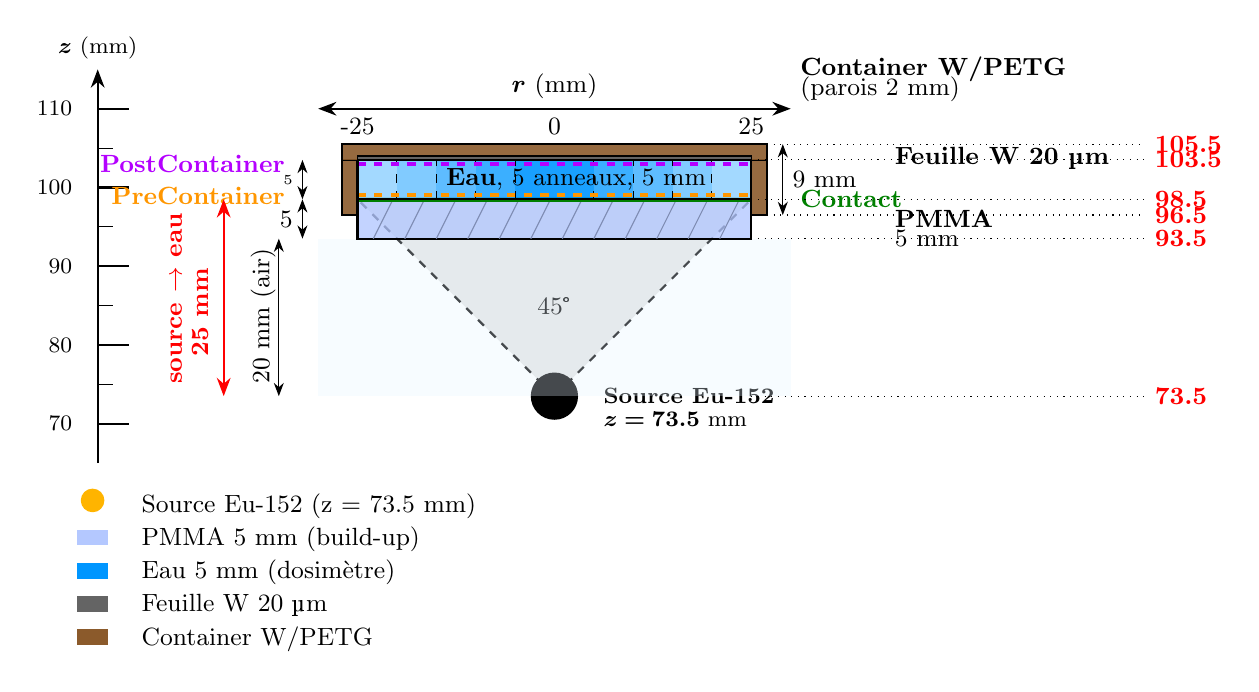
\begin{tikzpicture}[scale=0.1, >=Stealth]

    % ═══════════════════════════════════════════════════════════════════════════
    % DÉFINITION DES COULEURS
    % ═══════════════════════════════════════════════════════════════════════════
    \definecolor{sourcecolor}{RGB}{255, 180, 0}
    \definecolor{aircolor}{RGB}{230, 245, 255}
    \definecolor{pmmacolor}{RGB}{180, 200, 255}
    \definecolor{watercolor}{RGB}{0, 150, 255}
    \definecolor{tungstencolor}{RGB}{100, 100, 100}
    \definecolor{containercolor}{RGB}{139, 90, 43}
    \definecolor{precontainercolor}{RGB}{255, 150, 0}
    \definecolor{postcontainercolor}{RGB}{180, 0, 255}

    % ═══════════════════════════════════════════════════════════════════════════
    % AXE Z (vertical) avec graduations
    % ═══════════════════════════════════════════════════════════════════════════
		
    \draw[->, thick] (-58, 65) -- (-58, 115) node[above] {\footnotesize $\bm{z}$ (mm)};
    
    % Graduations principales
    \foreach \z in {70, 80, 90, 100, 110} {
        \draw[thick] (-58, \z) -- (-54, \z);
        \node[left] at (-60, \z) {\footnotesize \z};
    }
    
    % Graduations secondaires
    \foreach \z in {75, 85, 95, 105} {
        \draw (-58, \z) -- (-56, \z);
    }

    % ═══════════════════════════════════════════════════════════════════════════
    % SOURCE Eu-152 (z = 73.5 mm)
    % ═══════════════════════════════════════════════════════════════════════════
    \fill[black] (0, 73.5) circle (3);
    \node[black, right] at (5, 73.5) {\footnotesize \textbf{Source Eu-152}};
    \node[black, right] at (5, 70.5) {\footnotesize $\bm{z = 73.5}$ mm};
    
    % Cône d'émission (45°)
    % tan(45°) = 1, donc à z=98.5 (d=25), r = 25 mm
    \draw[black, dashed, thick] (0, 73.5) -- (-25, 98.5);
    \draw[black, dashed, thick] (0, 73.5) -- (25, 98.5);
    \fill[black, opacity=0.1] (0, 73.5) -- (-25, 98.5) -- (25, 98.5) -- cycle;
    \node[black] at (0, 85) {\small 45°};

    % ═══════════════════════════════════════════════════════════════════════════
    % AIR entre source et PMMA (z = 73.5 - 93.5 mm)
    % ═══════════════════════════════════════════════════════════════════════════
    \fill[aircolor, opacity=0.3] (-30, 73.5) rectangle (30, 93.5);
    
    % Annotation distance
    \draw[<->, thin, black] (-35, 73.5) -- (-35, 93.5);
    \node[black, left, rotate=90] at (-37, 93.5) {\small 20 mm (air)};

    % ═══════════════════════════════════════════════════════════════════════════
    % PMMA (z = 93.5 - 98.5 mm) - 5 mm
    % ═══════════════════════════════════════════════════════════════════════════
    \fill[pmmacolor, opacity=0.8] (-25, 93.5) rectangle (25, 98.5);
    \draw[black, thick] (-25, 93.5) rectangle (25, 98.5);
    
    % Hachures pour le PMMA
    \foreach \x in {-23,-19,...,23} {
        \draw[pmmacolor!70!black, thin] (\x, 93.5) -- (\x+2.5, 98.5);
    }
    
    \node[right] at (42, 96) {\small \textbf{PMMA}};
    \node[right] at (42, 93.5) {\small 5 mm};
    
    % Cotation PMMA
    \draw[<->, thin] (-32, 93.5) -- (-32, 98.5);
    \node[left] at (-32, 96) {\small 5};

    % ═══════════════════════════════════════════════════════════════════════════
    % INTERFACE PMMA/EAU - Contact direct (z = 98.5 mm)
    % ═══════════════════════════════════════════════════════════════════════════
    \draw[green!50!black, line width=2pt] (-25, 98.5) -- (25, 98.5);
    \node[green!50!black, right] at (30, 98.5) {\small \textbf{Contact}};

    % ═══════════════════════════════════════════════════════════════════════════
    % EAU - 5 anneaux concentriques (z = 98.5 - 103.5 mm)
    % ═══════════════════════════════════════════════════════════════════════════
    
    % Anneau 0 (r = 0-5 mm) - centre
    \fill[watercolor!100, opacity=0.9] (-5, 98.5) rectangle (5, 103.5);
    % Anneau 1 (r = 5-10 mm)
    \fill[watercolor!85, opacity=0.9] (-10, 98.5) rectangle (-5, 103.5);
    \fill[watercolor!85, opacity=0.9] (5, 98.5) rectangle (10, 103.5);
    % Anneau 2 (r = 10-15 mm)
    \fill[watercolor!70, opacity=0.9] (-15, 98.5) rectangle (-10, 103.5);
    \fill[watercolor!70, opacity=0.9] (10, 98.5) rectangle (15, 103.5);
    % Anneau 3 (r = 15-20 mm)
    \fill[watercolor!55, opacity=0.9] (-20, 98.5) rectangle (-15, 103.5);
    \fill[watercolor!55, opacity=0.9] (15, 98.5) rectangle (20, 103.5);
    % Anneau 4 (r = 20-25 mm)
    \fill[watercolor!40, opacity=0.9] (-25, 98.5) rectangle (-20, 103.5);
    \fill[watercolor!40, opacity=0.9] (20, 98.5) rectangle (25, 103.5);
    
    % Contour eau
    \draw[black, thick] (-25, 98.5) rectangle (25, 103.5);
    
    % Séparations des anneaux
    \foreach \r in {-20, -15, -10, -5, 5, 10, 15, 20} {
        \draw[black, thin, dashed] (\r, 98.5) -- (\r, 103.5);
    }
    
    \node[right] at (-15, 101) {\small \textbf{Eau}, 5 anneaux, 5 mm};

    % Cotation eau
    \draw[<->, thin] (-32, 98.5) -- (-32, 103.5);
    \node[left] at (-32, 101) {\tiny 5};

    % ═══════════════════════════════════════════════════════════════════════════
    % PLANS DE COMPTAGE (dans l'eau)
    % ═══════════════════════════════════════════════════════════════════════════
    
    % PreContainerPlane (z = 98.5 - 99.5 mm) - orange
    \draw[precontainercolor, line width=1.5pt, dashed] (-25, 99) -- (25, 99);
    \node[precontainercolor, left] at (-33, 99) {\small \textbf{PreContainer}};
    
    % PostContainerPlane (z = 102.5 - 103.5 mm) - violet
    \draw[postcontainercolor, line width=1.5pt, dashed] (-25, 103) -- (25, 103);
    \node[postcontainercolor, left] at (-33, 103) {\small \textbf{PostContainer}};

    % ═══════════════════════════════════════════════════════════════════════════
    % FEUILLE DE TUNGSTÈNE (z = 103.5 - 103.52 mm, 20 µm)
    % ═══════════════════════════════════════════════════════════════════════════
    \fill[tungstencolor] (-25, 103.5) rectangle (25, 104);  % Exagéré pour visibilité
    \draw[black] (-25, 103.5) rectangle (25, 104);
    \node[right] at (42, 103.75) {\small \textbf{Feuille W 20 µm}};

    % ═══════════════════════════════════════════════════════════════════════════
    % CONTAINER W/PETG (parois et couvercle)
    % Parois: r = 25-27 mm, z = 96.5 - 103.5 mm
    % Couvercle: r = 0-27 mm, z = 103.5 - 105.5 mm
    % ═══════════════════════════════════════════════════════════════════════════
    
    % Paroi gauche (r = 25-27 mm)
    \fill[containercolor, opacity=0.9] (-27, 96.5) rectangle (-25, 103.5);
    \draw[black, thick] (-27, 96.5) rectangle (-25, 103.5);
    
    % Paroi droite
    \fill[containercolor, opacity=0.9] (25, 96.5) rectangle (27, 103.5);
    \draw[black, thick] (25, 96.5) rectangle (27, 103.5);
    
    % Couvercle (z = 103.5 - 105.5 mm)
    \fill[containercolor, opacity=0.9] (-27, 103.5) rectangle (27, 105.5);
    \draw[black, thick] (-27, 103.5) -- (-27, 105.5) -- (27, 105.5) -- (27, 103.5);
    
    % La feuille W est DANS le container, redessinons-la au-dessus
    \fill[tungstencolor] (-25, 103.5) rectangle (25, 104);
    \draw[black, thin] (-25, 103.5) rectangle (25, 104);
    
    \node[right] at (30, 115) {\small \textbf{Container W/PETG}};
    \node[right] at (30, 112.5) {\small (parois 2 mm)};

    % Cotation container
    \draw[<->, thin] (29, 96.5) -- (29, 105.5);
    \node[right] at (29, 101) {\small 9 mm};

    % ═══════════════════════════════════════════════════════════════════════════
    % ANNOTATIONS DES POSITIONS Z
    % ═══════════════════════════════════════════════════════════════════════════
    
    % Lignes de repère à droite
    \draw[black, thin, dotted] (25, 73.5) -- (75, 73.5);
    \node[black, right] at (75, 73.5) {\small \color{red}\textbf{73.5}\color{black}};
    
    \draw[black, thin, dotted] (25, 93.5) -- (75, 93.5);
    \node[black, right] at (75, 93.5) {\small \color{red}\textbf{93.5}\color{black}};
    
    \draw[black, thin, dotted] (27, 96.5) -- (75, 96.5);
    \node[black, right] at (75, 96.5) {\small \color{red}\textbf{96.5}\color{black}};
    
    \draw[black, thin, dotted] (25, 98.5) -- (75, 98.5);
    \node[black, right] at (75, 98.5) {\small \color{red}\textbf{98.5}\color{black}};
    
    \draw[black, thin, dotted] (25, 103.5) -- (75, 103.5);
    \node[black, right] at (75, 103.5) {\small \color{red}\textbf{103.5}\color{black}};
    
    \draw[black, thin, dotted] (27, 105.5) -- (75, 105.5);
    \node[black, right] at (75, 105.5) {\small \color{red}\textbf{105.5}\color{black}};

    % ═══════════════════════════════════════════════════════════════════════════
    % AXE R (horizontal)
    % ═══════════════════════════════════════════════════════════════════════════
    \draw[<->, thick] (-30, 110) -- (30, 110);
    \node[above] at (0, 110) {\small $\bm{r}$ (mm)};
    \node[below] at (-25, 110) {\small -25};
    \node[below] at (0, 110) {\small 0};
    \node[below] at (25, 110) {\small 25};

    % ═══════════════════════════════════════════════════════════════════════════
    % COTATION DISTANCE SOURCE-EAU
    % ═══════════════════════════════════════════════════════════════════════════
    \draw[<->, thick, red] (-42, 73.5) -- (-42, 98.5);  %
    \node[red, left, rotate=90] at (-48, 98) {\small \textbf{source $\rightarrow$ eau}};
		\node[red, left, rotate=90] at (-45, 91) {\small \textbf{25 mm}};

    % ═══════════════════════════════════════════════════════════════════════════
    % LÉGENDE
    % ═══════════════════════════════════════════════════════════════════════════
    \node[anchor=north west] at (-64, 63) {
        \begin{tabular}{cl}
            \tikz\fill[sourcecolor] (0,0) circle (0.15); & \small Source Eu-152 (z = 73.5 mm) \\
            \tikz\fill[pmmacolor] (0,0) rectangle (0.4,0.2); & \small PMMA 5 mm (build-up) \\
            \tikz\fill[watercolor] (0,0) rectangle (0.4,0.2); & \small Eau 5 mm (dosimètre) \\
            \tikz\fill[tungstencolor] (0,0) rectangle (0.4,0.2); & \small Feuille W 20 µm \\
            \tikz\fill[containercolor] (0,0) rectangle (0.4,0.2); & \small Container W/PETG \\
        \end{tabular}
    };
\end{tikzpicture}
\captionsetup{labelformat=empty}
\caption{Coupe longitudinale du dispositif Puits Couronne \textbf{sans filtre}. La source Eu-152 est positionnée à $z = 73.5$ mm avec un cône d'émission de 45° (demi-angle). Le PMMA (5 mm) est en contact direct avec l'eau. Les 5 anneaux d'eau concentriques (nuances de bleu) permettent la mesure de dose radiale.}
\end{figure}

% Définition des couleurs
\definecolor{sourcecolor}{RGB}{255, 220, 150}
\definecolor{aircolor}{RGB}{230, 245, 255}
\definecolor{pmmacolor}{RGB}{200, 215, 255}
\definecolor{watercolor}{RGB}{180, 220, 255}
\definecolor{tungstencolor}{RGB}{200, 200, 200}
\definecolor{containercolor}{RGB}{220, 190, 160}
\definecolor{headercolor}{RGB}{70, 130, 180}

\medskip
\normalsize
\noindent \color{blue}\textbf{Distances caractéristiques}\color{black}
\footnotesize
\medskip

\begin{table}[h!]
\centering
\captionsetup{labelformat=empty}
\caption{\footnotesize Paramètres géométriques de la simulation}
\renewcommand{\arraystretch}{1.4}
\begin{tabular}{>{\columncolor{white}}l c c c c}
\toprule
\rowcolor{headercolor!30}
\footnotesize \textbf{Élément}&\footnotesize \textbf{Position z (mm)}&\footnotesize \textbf{Épaisseur}&\footnotesize \textbf{Rayon (mm)} &\footnotesize \textbf{Matériau} \\
\midrule
\rowcolor{sourcecolor!50}
\footnotesize Source Eu-152&\footnotesize 73.5&\footnotesize volumique &\footnotesize -- &\footnotesize  -- \\
\rowcolor{aircolor!50}
\footnotesize Air&\footnotesize 73.5 $\rightarrow$ 93.5&\footnotesize \SI{20}{mm}&\footnotesize  --&\footnotesize Air \\
\rowcolor{pmmacolor!50}
\footnotesize PMMA (build-up)&\footnotesize  93.5 $\rightarrow$ 98.5 &\footnotesize  \SI{5}{mm} &\footnotesize  25 &\footnotesize  PMMA \\
\rowcolor{watercolor!50}
\footnotesize Eau (dosimètre) &\footnotesize  98.5 $\rightarrow$ 103.5 &\footnotesize  \SI{5}{mm} &\footnotesize  25 &\footnotesize  G4\_WATER \\
\rowcolor{tungstencolor!50}
\footnotesize Feuille W &\footnotesize  103.5 $\rightarrow$ 103.52 &\footnotesize  \SI{20}{\micro m} &\footnotesize  25 &\footnotesize  G4\_W \\
\rowcolor{containercolor!50}
\footnotesize Parois container &\footnotesize  96.5 $\rightarrow$ 103.5 &\footnotesize  \SI{2}{mm} &\footnotesize  25--27 &\footnotesize  W/PETG (75\%/25\%) \\
\rowcolor{containercolor!50}
\footnotesize Couvercle container &\footnotesize  103.5 $\rightarrow$ 105.5 &\footnotesize  \SI{2}{mm} &\footnotesize  0--27 &\footnotesize  W/PETG (75\%/25\%) \\
\bottomrule
\end{tabular}
\end{table}

%===============================================================================
\normalsize
\noindent \begin{mdframed}[backgroundcolor=orange!20]
\subsection{\color{blue}\textbf{Analyse de la génération des événements}\color{black}}
\end{mdframed}
\footnotesize
%===============================================================================
\medskip


\normalsize
\noindent \color{blue}\textbf{Algorithme de génération}\color{black}
\footnotesize
\medskip

\begin{tcolorbox}[colback=blue!10,colframe=blue,title=\textbf{Principe}]
\noindent Dans cette simulation Geant4, chaque \color{blue}\textbf{événement}\color{black} \; correspond à une \color{blue}\textbf{désintégration}\color{black} du noyau d'Europium-152.\\
\noindent \color{blue}\textbf{Une désintégration peut émettre plusieurs photons gamma en cascade, chacun avec une probabilité d'émission indépendante}\color{black}
\end{tcolorbox}



\noindent Dans la simulation :
\begin{center}
\fbox{\textbf{1 événement Geant4 = 1 désintégration $^{152}$Eu}}
\end{center}

\noindent Chaque désintégration peut émettre \color{blue}\textbf{plusieurs photons gamma}\color{black} \;  de manière indépendante. Le nombre de photons émis par événement suit une distribution statistique déterminée par les intensités des raies.


\medskip 
\noindent Pour chaque événement (\color{blue}\textbf{désintégration}\color{black} \;), l'algorithme parcourt les $\bm{N} = 13$ raies et effectue \color{blue}\textbf{un tirage de Bernoulli indépendant pour chacune}\color{black} \; :












\begin{equation*}
\bm{\text{Pour chaque raie }} \bm{i} \in \{\bm{1}, \ldots, \bm{N}\} : \quad
\bm{\gamma_i} \bm{\text{ est émis si }} \quad \bm{\xi_i} < \bm{p_i}
\end{equation*}

\noindent où :
\begin{itemize}
\item $\bm{\xi_i} \sim \bm{\mathcal{U}(0,1)}$ est un nombre aléatoire uniforme sur $[0,1]$
\item $\bm{p_i} = \bm{I_i} / \bm{100}$ est la probabilité d'émission de la raie $\bm{i}$
\end{itemize}

\noindent Le nombre de photons émis par désintégration suit une \color{blue}\textbf{loi de Poisson composée}\color{black}. Chaque raie étant tirée indépendamment selon une loi de Bernoulli :\\

\begin{equation*}
\bm{n_\gamma} = \sum_{\bm{i}=\bm{1}}^{\bm{N}} \bm{X_i} \quad \bm{\text{avec}} \quad \bm{X_i} \sim \bm{\text{Bernoulli}}(\bm{p_i})
\end{equation*}

\noindent Le \color{blue}\textbf{nombre moyen de photons par désintégration}\color{black} \; est :\\

\begin{equation*}
\langle \bm{n_\gamma} \rangle = \sum_{\bm{i}=\bm{1}}^{\bm{N}} \bm{p_i} = \sum_{\bm{i}=\bm{1}}^{\bm{N}} \frac{\bm{I_i}}{\bm{100}} = \frac{\bm{202.78}}{\bm{100}} = \bm{2.0278}
\end{equation*}

\noindent La \color{blue}\textbf{variance}\color{black} \; est donnée par :\\

\begin{equation*}
\bm{\text{Var}}(\bm{n_\gamma}) = \sum_{\bm{i}=\bm{1}}^{\bm{N}} \bm{p_i} (\bm{1} - \bm{p_i}) = \sum_{\bm{i}=\bm{1}}^{\bm{N}} \bm{p_i} - \sum_{\bm{i}=\bm{1}}^{\bm{N}} \bm{p_i^2}
\end{equation*}

\noindent Numériquement, avec les valeurs du tableau  :\\

\begin{equation*}
\bm{\text{Var}}(\bm{n_\gamma}) = \bm{2.0278} - \bm{0.4126} = \bm{1.6152} \quad \Rightarrow \quad \bm{\sigma_{n_\gamma}} \approx \bm{1.27}
\end{equation*}
\medskip
\noindent Chaque photon est émis dans un cône d'ouverture $\bm{\theta_{\max}} = 45°$ orienté vers l'axe $\bm{+z}$. Pour obtenir une \color{blue}\textbf{distribution isotrope}\color{black} \; dans le cone, on utilise :\\

\begin{equation*}
\cos\bm{\theta} = \bm{1} - \bm{}\xi \cdot (\bm{1} - \cos\bm{\theta_{\max}})
\end{equation*}

\noindent où $\bm{\xi} \sim \bm{\mathcal{U}(0,1)}$.

\noindent L'angle azimutal est uniforme :\\

\begin{equation*}
\bm{\phi} = \bm{2\pi} \cdot \bm{\xi'}
\end{equation*}

\noindent où $\bm{\xi}' \sim \bm{\mathcal{U}}(0,1)$ est un second tirage indépendant.\\

\noindent Le vecteur direction unitaire est alors :

\begin{equation*}
\vec{\bm{u}} = \begin{pmatrix}
\sin\bm{\theta} \cos\bm{\phi} \\
\sin\bm{\theta} \sin\bm{\phi} \\
\cos\bm{\theta}
\end{pmatrix}
\end{equation*}

\noindent La fraction de l'angle solide $4\pi$ couverte par le cône est :

\begin{equation*}
\bm{f_\Omega} = \frac{\bm{\Omega}}{\bm{4\pi}} = \frac{\bm{2\pi}(\bm{1} - \cos\bm{\theta_{\max}})}{4\pi} = \frac{1 - \cos\theta_{\max}}{2}
\end{equation*}

\noindent Pour $\theta_{\max} = 45°$ :

\begin{equation*}
\bm{f_\Omega} = \frac{\bm{1} - \cos(45°)}{\bm{2}} = \frac{\bm{1} - \frac{\sqrt{\bm{2}}}{\bm{2}}}{\bm{2}} \approx \bm{0.1464} \approx \bm{14.6\%}
\end{equation*}
\medskip

\normalsize
\noindent \color{blue}\textbf{Résumé de l'implémentation}\color{black}
\footnotesize
\medskip
\begin{lstlisting}[language=C++, basicstyle=\small\ttfamily, frame=single, caption={\color{blue}Pseudo-code de la génération\color{black}}]
\textbf{Pour chaque evenement (desintegration):}
    n_gamma = 0
    Pour i = 0 a 12:  // 13 raies
        xi = random(0,1)
        Si xi < probabilite[i]:
            energie = energies[i]
            direction = generer_direction_cone(45 deg)
            emettre_gamma(energie, direction)
            n_gamma++
    \textbf{// n_gamma peut etre 0, 1, 2, 3, ...}
\end{lstlisting}

\normalsize
\noindent \color{blue}\textbf{Tableau des raies}\color{black}
\footnotesize
\medskip

% Définition des couleurs
\definecolor{headercolor}{RGB}{70, 130, 180}
\definecolor{xraycolor}{RGB}{255, 220, 180}
\definecolor{lowgamma}{RGB}{200, 230, 255}
\definecolor{midgamma}{RGB}{180, 255, 180}
\definecolor{highgamma}{RGB}{255, 200, 200}

\begin{table}[H]
\centering
\captionsetup{labelformat=empty}
\caption{\footnotesize Raies gamma et X de l'Eu-152 simulées (13 raies principales)}
\renewcommand{\arraystretch}{1.3}
\begin{tabular}{c c c c c}
\toprule
\rowcolor{headercolor!30}
\footnotesize \textbf{Index} &\footnotesize  \textbf{Énergie (keV)} &\footnotesize  \textbf{Intensité (\%)} &\footnotesize  \textbf{Type} &\footnotesize  \textbf{Origine} \\
\midrule
\rowcolor{xraycolor}
\footnotesize 0&\footnotesize 39.52&\footnotesize 20.8 &\footnotesize Raie X&\footnotesize  K$\alpha_2$ (Sm) \\
\rowcolor{xraycolor}
\footnotesize 1&\footnotesize 40.12&\footnotesize 37.7&\footnotesize Raie X&\footnotesize K$\alpha_1$ (Sm) \\
\rowcolor{lowgamma}
\footnotesize 2&\footnotesize 121.78&\footnotesize 28.41&\footnotesize$\gamma$&\footnotesize $^{152}$Sm$^*$ \\
\rowcolor{lowgamma}
\footnotesize 3&\footnotesize 244.70&\footnotesize 7.53&\footnotesize $\gamma$&\footnotesize $^{152}$Gd$^*$ \\
\rowcolor{midgamma}
\footnotesize 4&\footnotesize 344.28&\footnotesize 26.59&\footnotesize $\gamma$&\footnotesize $^{152}$Gd$^*$ \\
\rowcolor{midgamma}
\footnotesize 5&\footnotesize 411.12&\footnotesize 2.24&\footnotesize $\gamma$&\footnotesize $^{152}$Sm$^*$ \\
\rowcolor{midgamma}
\footnotesize 6&\footnotesize 443.97&\footnotesize 2.83&\footnotesize $\gamma$&\footnotesize $^{152}$Gd$^*$ \\
\rowcolor{midgamma}
\footnotesize 7&\footnotesize 778.90&\footnotesize 12.97&\footnotesize $\gamma$&\footnotesize $^{152}$Sm$^*$ \\
\rowcolor{midgamma}
\footnotesize 8&\footnotesize 867.38&\footnotesize 4.24&\footnotesize $\gamma$&\footnotesize $^{152}$Gd$^*$ \\
\rowcolor{midgamma}
\footnotesize 9&\footnotesize 964.08&\footnotesize 14.63&\footnotesize $\gamma$&\footnotesize $^{152}$Sm$^*$ \\
\rowcolor{highgamma}
\footnotesize  10&\footnotesize 1085.87&\footnotesize 10.21&\footnotesize $\gamma$&\footnotesize $^{152}$Sm$^*$ \\
\rowcolor{highgamma}
\footnotesize 11 &\footnotesize 1112.07&\footnotesize 13.64&\footnotesize $\gamma$& $^{152}$Sm$^*$ \\
\rowcolor{highgamma}
\footnotesize 12 &\footnotesize 1408.01&\footnotesize 21.01&\footnotesize $\gamma$&\footnotesize $^{152}$Sm$^*$ \\
\midrule
\multicolumn{2}{c}{\footnotesize \textbf{TOTAL}} &\footnotesize  \textbf{202.78} & & \\
\bottomrule
\end{tabular}
\end{table}

\noindent\textbf{Légende des couleurs :}
\begin{itemize}
\item \colorbox{xraycolor}{Raies X} : Fluorescence K du Samarium (E $<$ 50 keV)
\item \colorbox{lowgamma}{$\gamma$ basse énergie} : E $<$ 250 keV
\item \colorbox{midgamma}{$\gamma$ moyenne énergie} : 250 keV $<$ E $<$ 1000 keV
\item \colorbox{highgamma}{$\gamma$ haute énergie} : E $>$ 1000 keV
\end{itemize}

\medskip
\normalsize
\noindent \color{blue}\textbf{Vérification du nombre de gammas par désintégration}\color{black}
\footnotesize
\medskip

\begin{tcolorbox}[colback=blue!5,colframe=blue!50!black]
\begin{center}
\begin{tabular}{rl}
\footnotesize \textbf{Événements simulés :} &\footnotesize25 000 000 \\
\footnotesize \textbf{Primaires générés :} &\footnotesize 50 699 067 \\
\end{tabular}
\end{center}
\end{tcolorbox}

\noindent Le nombre moyen de gammas par désintégration est :

\begin{equation*}
\bm{\bar{n}_\gamma} = \frac{\bm{50\,699\,067}}{\bm{25\,000\,000}} = \bm{2.028}
\end{equation*}

\noindent Cette valeur correspond à la somme des intensités du spectre Eu-152 :

\begin{equation*}
\sum_{\bm{i}} \bm{I_i} = \bm{202.8}\% \implies \bm{\bar{n}_\gamma} = \bm{2.028} \quad \cmark
\end{equation*}

\begin{tcolorbox}[colback=blue!10,colframe=blue,title=\textbf{Conclusion}]
La génération des raies Eu-152 est \textbf{parfaitement cohérente}. Toutes les intensités sont reproduites avec une précision meilleure que 0.5\%.
\end{tcolorbox}

\medskip
\normalsize
\noindent \color{blue}\textbf{Vérification des intensités par raie}\color{black}
\footnotesize
\medskip

\begin{table}[H]
\centering
\captionsetup{labelformat=empty}
\caption{\footnotesize Comparaison des intensités simulées et attendues pour chaque raie Eu-152}
\renewcommand{\arraystretch}{1.2}
\begin{tabular}{c c c c c c}
\toprule
\rowcolor{headercolor!30}
\footnotesize \textbf{Raie (keV)}&\footnotesize \textbf{Émis}&\footnotesize \textbf{I simulée (\%)}&\footnotesize \textbf{I attendue (\%)}&\footnotesize \textbf{Écart}&\footnotesize \textbf{Statut} \\
\midrule
\footnotesize 39.52 (X)&\footnotesize 5 199 989&\footnotesize 20.80&\footnotesize 20.8&\footnotesize $<0.01\%$&\footnotesize \cmark \\
\footnotesize 40.12 (X)&\footnotesize 9 426 440&\footnotesize 37.71&\footnotesize 37.7&\footnotesize $<0.01\%$&\footnotesize \cmark \\
\footnotesize 121.78&\footnotesize 7 099 951&\footnotesize 28.40&\footnotesize 28.41&\footnotesize $<0.01\%$&\footnotesize \cmark \\
\footnotesize 244.70&\footnotesize 1 882 297&\footnotesize 7.53&\footnotesize 7.53&\footnotesize $<0.01\%$&\footnotesize \cmark \\
\footnotesize 344.28&\footnotesize 6 649 673&\footnotesize 26.60&\footnotesize 26.59&\footnotesize $<0.01\%$&\footnotesize \cmark \\
\footnotesize 411.12&\footnotesize 558 246&\footnotesize 2.23&\footnotesize 2.24&\footnotesize $<0.5\%$&\footnotesize \cmark \\
\footnotesize 443.97&\footnotesize 706 678&\footnotesize 2.83&\footnotesize 2.83&\footnotesize $<0.01\%$&\footnotesize \cmark \\
\footnotesize 778.90&\footnotesize 3 245 196&\footnotesize 12.98&\footnotesize 12.97&\footnotesize $<0.1\%$&\footnotesize \cmark \\
\footnotesize 867.38&\footnotesize 1 060 009&\footnotesize 4.24&\footnotesize 4.24&\footnotesize $<0.01\%$&\footnotesize \cmark \\
\footnotesize 964.08&\footnotesize 3 658 532&\footnotesize 14.63&\footnotesize 14.63&\footnotesize $<0.01\%$& \cmark \\
\footnotesize 1085.87&\footnotesize 2 551 198&\footnotesize 10.20&\footnotesize 10.21&\footnotesize $<0.1\%$&\footnotesize \cmark \\
\footnotesize 1112.07&\footnotesize 3 409 096&\footnotesize 13.64&\footnotesize 13.64&\footnotesize $<0.01\%$&\footnotesize \cmark \\
\footnotesize 1408.01&\footnotesize 5 251 762&\footnotesize 21.01&\footnotesize 21.01&\footnotesize $<0.01\%$&\footnotesize \cmark \\
\midrule
\footnotesize\textbf{TOTAL} &\footnotesize \textbf{50 699 067} &\footnotesize \textbf{202.80} &\footnotesize \textbf{202.78} &\footnotesize $<0.01\%$ &\footnotesize \cmark \\
\bottomrule
\end{tabular}
\end{table}


%===============================================================================
\normalsize
\noindent \begin{mdframed}[backgroundcolor=orange!20]
\subsection{\color{blue}\textbf{Angle Solide}\color{black}}
\end{mdframed}
\footnotesize
%===============================================================================
\medskip

\normalsize
\noindent \color{blue}\textbf{Définition de l'angle solide}\color{black}
\footnotesize
\medskip

\noindent L'angle solide $\bm{\Omega}$ est la mesure bidimensionnelle de la portion de sphère vue  depuis un point. Pour une sphère complète :

\begin{equation*}
\bm{\Omega_{4\pi}} = \bm{4\pi} \text{ sr (stéradians)}
\end{equation*}

\noindent Pour un cône de demi-angle $\bm{\theta_0}$ autour de l'axe $\bm{z}$, l'angle solide est :

\begin{equation*}
\bm{\Omega_{\text{cône}}} = \int_{\bm{0}}^{\bm{2\pi}} \bm{d\phi} \int_0^{\bm{\theta_0}} \sin\bm{\theta} \, \bm{d\theta} = \bm{2\pi} (\bm{1} - \cos\bm{\theta_0})
\end{equation*}

\noindent Avec un demi-angle $\bm{\theta_0} = \bm{45}^{\circ}$ :

\begin{equation*}
\bm{\Omega_{\text{cône}}} = \bm{2\pi} (\bm{1 }- \cos \bm{45}^{\circ}) = \bm{2\pi} (\bm{1} - \bm{0.707}) = \bm{2\pi} \times \bm{0.293} = \bm{1.84} \text{ sr}
\end{equation*}

\noindent La \color{blue}\textbf{fraction d'angle solide}\color{black} couverte par le cône est :

\begin{equation*}
\bm{f_\Omega} = \frac{\bm{\Omega_{\text{cône}}}}{\bm{4\pi}} = \frac{\bm{1} - \cos\bm{\theta_0}}{\bm{2}} = \frac{\bm{1} - \cos \bm{45}^{\circ}}{\bm{2}} = \bm{0.146} = \bm{14.6}\%
\end{equation*}

\medskip
\normalsize
\noindent \color{blue}\textbf{Géométrie des angles solides}\color{black}
\footnotesize
\medskip

\begin{figure}[H]
\centering
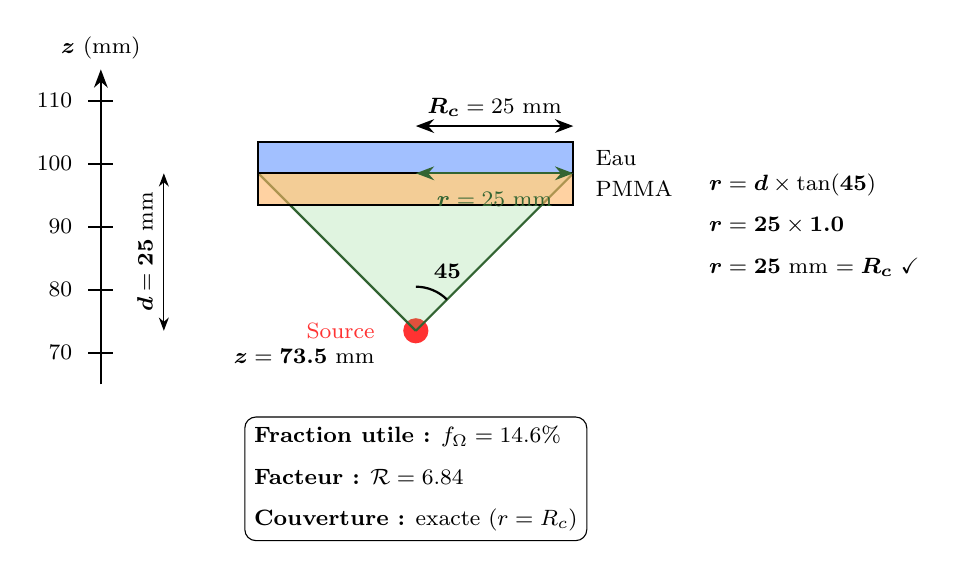
\begin{tikzpicture}[scale=0.08, >=Stealth]

    % ═══════════════════════════════════════════════════════════════════════════
    % AXE Z
    % ═══════════════════════════════════════════════════════════════════════════
    
    \draw[->, thick] (-50, 65) -- (-50, 115) node[above] {\footnotesize $\bm{z}$ (mm)};
    \foreach \z in {70, 80, 90, 100, 110} {
        \draw[thick] (-52, \z) -- (-48, \z);
        \node[left] at (-53, \z) {\footnotesize \z};
    }
    
    % ═══════════════════════════════════════════════════════════════════════════
    % SOURCE
    % ═══════════════════════════════════════════════════════════════════════════
    
    \fill[sourcecolor] (0, 73.5) circle (2);
    \node[sourcecolor, left] at (-5, 73.5) {\footnotesize Source};
    \node[left] at (-5, 69.5) {\footnotesize $\bm{z} = \bm{73.5}$ mm};
    
    % ═══════════════════════════════════════════════════════════════════════════
    % CÔNE D'ÉMISSION
    % ═══════════════════════════════════════════════════════════════════════════
    
    % tan(45°) = 1.0, à d=25mm : r = 25mm
    \fill[usefulcolor, opacity=0.2] (0, 73.5) -- (-25, 98.5) -- (25, 98.5) -- cycle;
    \draw[usefulcolor!50!black, thick] (0, 73.5) -- (-25, 98.5);
    \draw[usefulcolor!50!black, thick] (0, 73.5) -- (25, 98.5);
    
    % Angle
    \draw[thick] (0, 80.5) arc (90:45:7);
    \node at (5, 83) {\footnotesize $\bm{45}°$};
    
    % ═══════════════════════════════════════════════════════════════════════════
    % PMMA
    % ═══════════════════════════════════════════════════════════════════════════
    
    \fill[pmmacolor, opacity=0.6] (-25, 93.5) rectangle (25, 98.5);
    \draw[black, thick] (-25, 93.5) rectangle (25, 98.5);
    \node[right] at (27, 96) {\footnotesize PMMA};
    
    % ═══════════════════════════════════════════════════════════════════════════
    % EAU
    % ═══════════════════════════════════════════════════════════════════════════
    
    \fill[watercolor, opacity=0.6] (-25, 98.5) rectangle (25, 103.5);
    \draw[black, thick] (-25, 98.5) rectangle (25, 103.5);
    \node[right] at (27, 101) {\footnotesize Eau};
    
    % Parois
    \draw[black, thick] (-25, 93.5) -- (-25, 103.5);
    \draw[black, thick] (25, 93.5) -- (25, 103.5);
    
    % ═══════════════════════════════════════════════════════════════════════════
    % RAYONS
    % ═══════════════════════════════════════════════════════════════════════════
    
    % Rayon container
    \draw[<->, thick] (0, 106) -- (25, 106);
    \node[above] at (12.5, 106) {\footnotesize $\bm{R_c} = 25$ mm};
    
    % Rayon cône (= rayon container à z=98.5)
    \draw[<->, usefulcolor!50!black, thick] (0, 98.5) -- (25, 98.5);
    \node[usefulcolor!50!black, below] at (12.5, 97) {\footnotesize $\bm{r} = 25$ mm};
    
    % Distance source -> eau
    \draw[<->, black] (-40, 73.5) -- (-40, 98.5);
    \node[black, rotate=90] at (-43, 86) {\footnotesize $\bm{d} = \bm{25}$ mm};
    
    % ═══════════════════════════════════════════════════════════════════════════
    % FORMULES
    % ═══════════════════════════════════════════════════════════════════════════
    
    \node[anchor=north west, align=left] at (45, 100) {
        \footnotesize $\bm{r} = \bm{d} \times \tan(\bm{45}°)$\\[3pt]
        \footnotesize $\bm{r} = \bm{25} \times \bm{1.0}$\\[3pt]
        \footnotesize $\bm{r} = \bm{25}$ mm $= \bm{R_c}$ \checkmark
    };
    
    % ═══════════════════════════════════════════════════════════════════════════
    % ENCADRÉ
    % ═══════════════════════════════════════════════════════════════════════════
    
    \node[draw, fill=white, rounded corners, align=left] at (0, 50) {
        \footnotesize \textbf{Fraction utile :} $f_\Omega = 14.6\%$\\[3pt]
        \footnotesize \textbf{Facteur :} $\mathcal{R} = 6.84$\\[3pt]
        \footnotesize \textbf{Couverture :} exacte ($r = R_c$)
    };

\end{tikzpicture}
\captionsetup{labelformat=empty}
\caption{\footnotesize Géométrie du cône d'émission. Le cône de 45° couvre exactement le rayon du container (25 mm) au niveau de l'entrée de l'eau. La couverture est optimale.}
\end{figure}

\begin{center}
\fbox{
\parbox{0.85\textwidth}{
\centering
\textbf{\large \color{blue}\textbf{Angle solide et renormalisation}\color{black}}\\[10pt]

\begin{tabular}{rl}
\color{blue}\textbf{Problème :}\color{black} & Une source réelle émet dans toutes les directions ($\bm{4\pi}$)\\[3pt]
& $\Rightarrow$ La plupart des gammas ne touchent pas le détecteur\\[8pt]

\color{blue}\textbf{Solution :}\color{black} & Simuler uniquement un cône dirigé vers le détecteur\\[3pt]
& $\Rightarrow$ Gain de temps de calcul considérable\\[8pt]

\color{blue}\textbf{Fraction utile :}\color{black}& $\bm{f_\Omega} = \dfrac{\bm{1} - \cos(\bm{45}°)}{2} = \bm{14.6}\%$\\[10pt]

\color{blue}\textbf{Équivalence :}\color{black}& 1 evt simulation = 0.146 désintégration réelle\\[3pt]
& 6.84 evt simulation = 1 désintégration réelle\\[8pt]

\color{blue}\textbf{Conversion dose :}\color{black}& $\bm{D_{\text{réelle}}} = \bm{D_{\text{simulation}}} \times 0.146$\\[8pt]

\color{blue}\textbf{Temps irradiation :}\color{black}& $\bm{t} = \dfrac{\bm{N_{\text{evt}}} \times \bm{6.84}}{\bm{A}}$ (avec $\bm{A}$ en Bq)
\end{tabular}
}
}
\end{center}

\medskip
\normalsize
\noindent \color{blue}\textbf{Vérification de la couverture géométrique}\color{black}
\footnotesize
\medskip

\noindent Le rayon couvert par le cône à la distance $\bm{d}$ de la source est :

\begin{equation*}
\bm{r_{\text{cône}}}(\bm{d}) = \bm{d} \times \tan\bm{\theta_0}
\end{equation*}

\begin{table}[H]
\centering
\captionsetup{labelformat=empty}
\caption{\footnotesize Rayon couvert par le cône ($\theta_0 = 45^{\circ}$) à différentes positions}
\begin{tabular}{@{}l c c c c@{}}
\toprule
\footnotesize\textbf{Position}&\footnotesize $z$ \textbf{(mm)}&\footnotesize $d = z - z_s$ \textbf{(mm)}&\footnotesize $r_{\text{cône}}$ \textbf{(mm)}&\footnotesize \textbf{Couverture} \\
\midrule
\footnotesize Bas PMMA&\footnotesize 93.5&\footnotesize 20.0&\footnotesize 20.0&\footnotesize $< R_c$ \\
\rowcolor{watercolor!20}
\footnotesize Bas eau&\footnotesize 98.5&\footnotesize 25.0&\footnotesize \textbf{25.0}&\footnotesize $= R_c$ \\
\footnotesize Centre eau&\footnotesize 101.0&\footnotesize 27.5&\footnotesize 27.5&\footnotesize $> R_c$  \\
\footnotesize Haut eau &\footnotesize 103.5&\footnotesize 30.0&\footnotesize 30.0&\footnotesize $> R_c$  \\
\bottomrule
\end{tabular}
\end{table}

\begin{tcolorbox}[colback=blue!5,colframe=blue,title=\textbf{Conclusion}]
\noindent Le cône de $45^{\circ}$ couvre exactement le container d'eau ($\bm{R_c} = 25$ mm) à l'entrée de l'eau ($z = 98.5$ mm), puis dépasse dans l'épaisseur de l'eau avec une marge croissante jusqu'à $+5$ mm en sortie.
\end{tcolorbox}

%===============================================================================
\normalsize
\noindent \begin{mdframed}[backgroundcolor=orange!20]
\subsection{\color{blue}\textbf{Renormalisation du temps d'irradiation}\color{black}}
\end{mdframed}
\footnotesize
%===============================================================================
\medskip

\medskip
\normalsize
\noindent \color{blue}\textbf{Paramètres de la simulation}\color{black}
\footnotesize
\medskip

\begin{table}[H]
\centering
\captionsetup{labelformat=empty}
\caption{\footnotesize Paramètres de normalisation}
\begin{tabular}{@{}lcc@{}}
\toprule
\footnotesize \textbf{Paramètre} &\footnotesize \textbf{Symbole} &\footnotesize \textbf{Valeur} \\
\midrule
\footnotesize Activité source (4$\pi$) &\footnotesize $A_{4\pi}$ &\footnotesize 42 kBq \\
\footnotesize Demi-angle du cône &\footnotesize $\theta_{\max}$ &\footnotesize 45° \\
\footnotesize Fraction d'angle solide &\footnotesize $f_\Omega$ &\footnotesize 14.6\% \\
\footnotesize Activité effective (cône) &\footnotesize $A_{\text{eff}}$ &\footnotesize 6.15 kBq \\
\footnotesize Photons moyens/désintégration &\footnotesize $\langle n_\gamma \rangle$ &\footnotesize 2.03 \\
\footnotesize Position source &\footnotesize $z_s$ &\footnotesize 73.5 mm \\
\bottomrule
\end{tabular}
\end{table}

\medskip
\normalsize
\noindent \color{blue}\textbf{Résumé des Constantes dans le Code}\color{black}
\footnotesize
\medskip

\begin{table}[H]
\centering
\captionsetup{labelformat=empty}
\caption{\footnotesize Correspondance code/physique}
\begin{tabular}{@{}lll@{}}
\toprule
\footnotesize \textbf{Variable C++} &\footnotesize \textbf{Valeur} &\footnotesize \textbf{Signification} \\
\midrule
\footnotesize \texttt{GetMeanGammasPerDecay()} &\footnotesize 2.03 &\footnotesize $\langle n_\gamma \rangle$ \\
\footnotesize \texttt{fMeanGammasPerDecay} &\footnotesize 2.03 &\footnotesize Idem (RunAction) \\
\footnotesize \texttt{fActivity4pi} &\footnotesize 4.2$\times 10^4$ &\footnotesize $A_{4\pi}$ en Bq \\
\footnotesize \texttt{fConeAngle} &\footnotesize 45° & $\theta_{\max}$ \\
\footnotesize \texttt{GetSolidAngleFraction()} &\footnotesize 0.146 &\footnotesize $f_\Omega$ \\
\footnotesize \texttt{kNbGammaLines} &\footnotesize 13 &\footnotesize Nombre de raies \\
\bottomrule
\end{tabular}
\end{table}

\medskip
\normalsize
\noindent \color{blue}\textbf{Relation avec l'activité}\color{black}
\footnotesize
\medskip

\noindent L'activité de la source sur $\bm{4\pi}$ est $\bm{A_{4\pi}} = \SI{42}{kBq}$. L'activité effective dans le cône est :

\begin{equation*}
\bm{A_{\text{eff}}} = \bm{A_{4\pi}} \times \bm{f_\Omega} \approx \bm{42} \times \bm{0.1464} \approx \SI{6.15}{kBq}
\end{equation*}

\noindent La correspondance entre le nombre d'événements simulés $\bm{N_{\text{evt}}}$ et le temps d'irradiation $\bm{t_{\text{irr}}}$ est :

\begin{equation*}
\bm{t_{\text{irr}}} = \frac{\bm{N_{\text{evt}}}}{\bm{A_{4\pi}} \times \bm{f_\Omega}}
\end{equation*}

\noindent où $\bm{f_\Omega}$ est la fraction d'angle solide couverte par le cône d'émission.

\medskip
\normalsize
\noindent \color{blue}\textbf{Temps d'irradiation équivalent}\color{black}\\
\footnotesize
\medskip
\noindent Un événement de simulation correspond à une désintégration dans le cône. Le temps d'irradiation équivalent à $\bm{N_{\text{evt}}}$ événements simulés est :

\begin{equation*}
\bm{t_{\text{irr}}} = \frac{\bm{N_{\text{evt}}}}{\bm{A_{\text{eff}}}} = \frac{\bm{N_{\text{evt}}}}{\bm{A_{4\pi}} \times \bm{f_\Omega}}
\end{equation*}


\noindent Pour $\bm{N_{\text{evt}}}$ événements simulés, le temps d'irradiation équivalent est :\\

\begin{equation*}
\boxed{\bm{t_{\text{irr}}} = \frac{\bm{N_{\text{evt}}}}{\bm{A_{4\pi}} \times \bm{f_\Omega}} = \frac{\bm{N_{\text{evt}}}}{\bm{42000} \times \bm{0.146}} \text{ s} = \frac{\bm{N_{\text{evt}}}}{\bm{6132}} \text{ s}}
\end{equation*}

\medskip
\normalsize
\noindent \color{blue}\textbf{Calcul du débit de dose}\color{black}
\footnotesize
\medskip

\noindent Si $\bm{D_{\text{sim}}}$ est la dose totale simulée (en Gy) pour $\bm{N_{\text{evt}}}$ événements :

\begin{equation*}
\boxed{\bm{\dot{D}} = \frac{\bm{D_{\text{sim}}}}{\bm{t_{\text{irr}}}} = \frac{\bm{D_{\text{sim}} }\times \bm{A_{4\pi}} \times \bm{f_\Omega}}{\bm{N_{\text{evt}}}}}
\end{equation*}

\noindent En nGy/s :

\begin{equation*}
\bm{\dot{D}} \text{ (nGy/s)} = \frac{\bm{D_{\text{sim}}} \text{ (nGy)}}{\bm{N_{\text{evt}}}} \times \bm{6132}
\end{equation*}

\normalsize
\noindent \color{blue}\textbf{Application aux doses}\color{black}\\
\footnotesize
\medskip
\noindent La dose par désintégration réelle est :
\begin{equation*}
\bm{D_{\text{réel}}} = \bm{D_{\text{sim}}} \times \bm{f_\Omega} = \frac{\bm{D_{\text{sim}}}}{\bm{\mathcal{R}}}
\end{equation*}
\medskip
\normalsize
\noindent \color{blue}\textbf{Schéma récapitulatif}\color{black}
\footnotesize
\medskip

\begin{figure}[H]
\centering
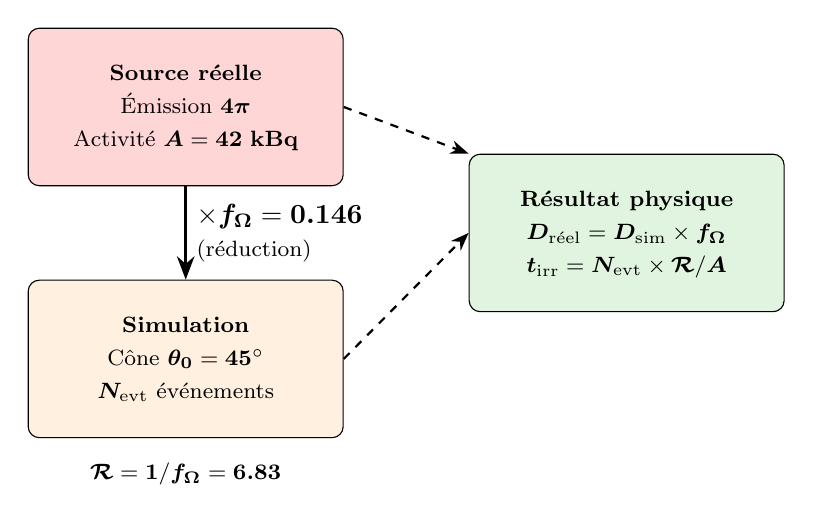
\begin{tikzpicture}[>=Stealth, scale=0.8]
    
    % Boîte source 4\pi
    \node[draw, fill=sourcecolor!20, minimum width=4cm, minimum height=2cm, rounded corners] (source4pi) at (0, 4) {
        \begin{tabular}{c}
            \footnotesize \textbf{Source réelle}\\
            \footnotesize Émission $\bm{4\pi}$\\
            \footnotesize Activité $\bm{A} = \bm{42}$ \textbf{kBq}
        \end{tabular}
    };
    
    % Boîte simulation cône
    \node[draw, fill=conecolor!20, minimum width=4cm, minimum height=2cm, rounded corners] (simcone) at (0, 0) {
        \begin{tabular}{c}
            \footnotesize \textbf{Simulation}\\
            \footnotesize Cône $\bm{\theta_0} = \bm{45}^{\circ}$\\
            \footnotesize $\bm{N_{\text{evt}}}$ \footnotesize événements
        \end{tabular}
    };
    
    % Flèche avec facteur
    \draw[->, very thick] (source4pi) -- (simcone) node[midway, right, align=left] {
        $\times \bm{f_\Omega} = \bm{0.146}$\\
        \footnotesize (réduction)
    };
    
    % Boîte résultat
    \node[draw, fill=solidanglecolor!20, minimum width=4cm, minimum height=2cm, rounded corners] (result) at (7, 2) {
        \begin{tabular}{c}
            \footnotesize \textbf{Résultat physique}\\
            \footnotesize $\bm{D_{\text{réel}}} = \bm{D_{\text{sim}}} \times \bm{f_\Omega}$\\
            \footnotesize $\bm{t_{\text{irr}}} = \bm{N_{\text{evt}}} \times \bm{\mathcal{R}} / \bm{A}$
        \end{tabular}
    };
    
    % Flèches vers résultat
    \draw[->, thick, dashed] (simcone.east) -- (result.west);
    \draw[->, thick, dashed] (source4pi.east) -- (result.north west);
    
    % Annotation
    \node[below] at (0, -1.5) {\footnotesize $\bm{\mathcal{R}} = \bm{1}/\bm{f_\Omega} = \bm{6.83}$};
\end{tikzpicture}
\captionsetup{labelformat=empty}
\caption{\footnotesize Schéma de renormalisation entre simulation (cône) et source réelle ($\bm{4\pi}$).}
\end{figure}

\medskip
\normalsize
\noindent \color{blue}\textbf{Application numérique}\color{black}
\footnotesize
\medskip

\noindent Pour $\bm{N_{\text{evt}}} = \bm{25} \times \bm{10^6}$ événements simulés :\\

\begin{itemize}
\item Nombre de désintégrations $\bm{4\pi}$ représentées : $\bm{N_{\text{désint}}} = \bm{N_{\text{evt}}} \times \bm{\mathcal{R}} = \bm{25} \times \bm{10^6} \times \bm{6.83} = \bm{171} \times \bm{10^6}$
\item Temps d'irradiation simulé : $\bm{t_{\text{irr}}} = \frac{\bm{N_{\text{désint}}}}{\bm{A}} = \frac{\bm{171} \times \bm{10^6}}{\bm{42} \times \bm{10^3}} = \bm{4071}$ s $\approx$ \textbf{68 min}
\end{itemize}

\medskip
\noindent Le débit de dose est calculé par :
\begin{equation*}
\bm{\dot{D}} = \bm{D_{\text{sim}}} \times \bm{A_{\text{eff}}} = \frac{\bm{D_{\text{sim}}}}{\bm{N_{\text{evt}}}} \times \bm{A} \times \bm{f_\Omega}
\end{equation*}

\clearpage

%===============================================================================
\normalsize
\noindent \begin{mdframed}[backgroundcolor=orange!20]
\subsection{\color{blue}\textbf{Relations activité--temps d'irradiation}\color{black}}
\end{mdframed}
\footnotesize
%===============================================================================

\medskip
\normalsize
\noindent \color{blue}\textbf{Définitions}\color{black}
\footnotesize
\medskip

\medskip
\normalsize
\noindent \color{blue}\textbf{Calcul du temps d'irradiation}\color{black}
\footnotesize
\medskip

\begin{itemize}
\item \textbf{Activité source ($\bm{4\pi}$)} : $\bm{A_{4\pi}} = \SI{42}{kBq}$ = \textbf{42\,000} désintégrations/s
\item \textbf{Activité effective} (dans le cône) : $\bm{A_{\text{eff}}} = \bm{A_{4\pi}} \times \bm{f_\Omega}$
\end{itemize}

\begin{equation*}
\bm{A_{\text{eff}}} = \bm{A_{4\pi}} \times \bm{f_\Omega} = \bm{42\,000} \times \bm{0.1464} = \SI{6149}{Bq} \approx \SI{6.15}{kBq}
\end{equation*}

\noindent Dans la simulation :
\begin{center}
1 événement Geant4 = 1 désintégration dans le cône
\end{center}

\noindent Le temps d'irradiation équivalent à $\bm{N_{\text{evt}}}$ événements simulés est :

\begin{equation*}
\bm{t_{\text{irr}}} = \frac{\bm{N_{\text{evt}}}}{\bm{A_{\text{eff}}}} = \frac{\bm{N_{\text{evt}}}}{\bm{A_{4\pi}} \times \bm{f_\Omega}}
\end{equation*}

\textbf{Application numérique} pour $\bm{N_{\text{evt}}} = 25 \times 10^6$ :

\begin{equation*}
\bm{t_{\text{irr}}} = \frac{\bm{25} \times \bm{10^6}}{\bm{6149}} = \SI{4066}{s} = \SI{67.8}{min} \approx \SI{1.13}{h}
\end{equation*}

\medskip
\normalsize
\noindent \color{blue}\textbf{Formule inverse}\color{black}\par
\footnotesize
\medskip

\noindent Pour atteindre un temps d'irradiation $t$ donné, le nombre d'événements requis est :

\begin{equation}
\bm{N_{\text{evt}}} = \bm{A_{\text{eff}}} \times \bm{t} = \bm{A_{4\pi}} \times \bm{f_\Omega} \times \bm{t}
\end{equation}

\begin{table}[H]
\centering
\captionsetup{labelformat=empty}
\caption{Correspondance temps -- nombre d'événements}
\begin{tabular}{@{}ccc@{}}
\toprule
\footnotesize\textbf{\footnotesize Temps d'irradiation} &\footnotesize \textbf{Nombre d'événements} &\footnotesize \textbf{Note} \\
\midrule
\footnotesize \SI{1}{h} &\footnotesize $2.21 \times 10^7$ &\footnotesize $\approx$ 22 millions \\
\footnotesize \SI{1}{jour} &\footnotesize $5.31 \times 10^8$ &\footnotesize $\approx$ 531 millions \\
\footnotesize \SI{1}{semaine} &\footnotesize $3.72 \times 10^9$ &\footnotesize $\approx$ 3.7 milliards \\
\bottomrule
\end{tabular}
\end{table}

%===============================================================================
\normalsize
\noindent \begin{mdframed}[backgroundcolor=orange!20]
\subsection{\color{blue}\textbf{Analyse du Débit de Dose}\color{black}}
\end{mdframed}
\footnotesize
%===============================================================================
\medskip

\normalsize
\noindent \color{blue}\textbf{Formule de calcul}\color{black}
\footnotesize
\medskip

\noindent Le débit de dose $\bm{\dot{D}}$ est calculé à partir de la dose par événement simulé :

\begin{equation*}
\bm{\dot{D}} = \frac{\bm{D_{\text{sim}}}}{\bm{N_{\text{evt}}}} \times \bm{A_{\text{eff}}} = \frac{\bm{D_{\text{sim}}}}{\bm{N_{\text{evt}}}} \times \bm{A_{4\pi}} \times \bm{f_\Omega}
\end{equation*}

\noindent En développant les unités :

\begin{equation*}
\bm{\dot{D}} \, [\si{nGy/s}] = \bm{D_{\text{evt}}} \, [\si{nGy}] \times \bm{A_{\text{eff}}} \, [\si{Bq}]
\end{equation*}

\noindent Pour convertir en \si{\micro Gy/h} :

\begin{equation*}
\bm{\dot{D}} \, [\si{\micro Gy/h}] = \bm{D_{\text{evt}}} \, [\si{nGy}] \times \bm{A_{\text{eff}}} \, [\si{Bq}] \times \frac{\bm{3600}}{\bm{1000}}
\end{equation*}

\medskip
\normalsize
\noindent \color{blue}\textbf{Résultats par anneau d'eau}\color{black}
\footnotesize
\medskip

\begin{table}[H]
\centering
\captionsetup{labelformat=empty}
\caption{\footnotesize Débit de dose par anneau (source Eu-152, 42 kBq)}
\begin{tabular}{@{}ccccccc@{}}
\toprule
\footnotesize \textbf{Anneau} &\footnotesize \textbf{Rayon} &\footnotesize \textbf{Masse} &\footnotesize \textbf{Dose/evt} &\footnotesize \textbf{Débit} &\footnotesize \textbf{t(20 cGy)} &\footnotesize \textbf{t(20 cGy)} \\
 &\footnotesize \textbf{(mm)} &\footnotesize \textbf{(g)} &\footnotesize \textbf{(nGy)} &\footnotesize \textbf{(\si{\micro Gy/h})} &\footnotesize \textbf{(h)} &\footnotesize \textbf{(jours)} \\
\midrule
\footnotesize 0 &\footnotesize 0--5 &\footnotesize 0.393 &\footnotesize $2.87 \times 10^{-4}$ &\footnotesize 6.35 &\footnotesize 31\,485 &\footnotesize 1\,312 \\
\footnotesize 1 &\footnotesize 5--10 &\footnotesize 1.178 &\footnotesize $2.71 \times 10^{-4}$ &\footnotesize 6.00 &\footnotesize 33\,362 &\footnotesize 1\,390 \\
\footnotesize 2 &\footnotesize 10--15 &\footnotesize 1.964 &\footnotesize $2.40 \times 10^{-4}$ &\footnotesize 5.32 &\footnotesize 37\,602 &\footnotesize 1\,567 \\
\footnotesize 3 &\footnotesize 15--20 &\footnotesize 2.749 &\footnotesize $2.06 \times 10^{-4}$ &\footnotesize 4.56 &\footnotesize 43\,908 &\footnotesize 1\,830 \\
\footnotesize 4 &\footnotesize 20--25 &\footnotesize 3.534 &\footnotesize $1.82 \times 10^{-4}$ &\footnotesize 4.02 &\footnotesize 49\,754 &\footnotesize 2\,073 \\
\midrule
\footnotesize \textbf{Total} &\footnotesize 0--25 &\footnotesize 9.817 &\footnotesize $2.15 \times 10^{-4}$ &\footnotesize 26.24 &\footnotesize 7\,622 & 318 \\
\bottomrule
\end{tabular}
\end{table}

\medskip
\normalsize
\noindent \color{blue}\textbf{Analyse de l'anneau central (Anneau 0)}\color{black}
\footnotesize
\medskip

\noindent L'anneau central ($\bm{r} = 0$--$5$ mm) reçoit le \textbf{débit de dose le plus élevé} :

\begin{equation*}
\bm{\dot{D}_{\text{anneau 0}}} = \SI{6.35}{\micro Gy/h} = \SI{0.00635}{mGy/h}
\end{equation*}

\medskip
\normalsize
\noindent \color{blue}\textbf{Vérification du calcul}\color{black}
\footnotesize
\medskip

\begin{align*}
\bm{D_{\text{evt}}} &= \SI{2.869e-4}{nGy} \quad \text{(dose par événement simulé)} \\
\bm{A_{\text{eff}}} &= \SI{6149}{Bq} \\
\bm{\dot{D}} &= \bm{D_{\text{evt}}} \times \bm{A_{\text{eff}}} = \bm{2.869} \times \bm{10^{-4}} \times \bm{6149} = \SI{1.764}{nGy/s} \\
\bm{\dot{D}} &= \bm{1.764 }\times \bm{3.6} = \SI{6.35}{\micro Gy/h} \quad \checkmark
\end{align*}

\medskip
\normalsize
\noindent \color{blue}\textbf{Temps d'irradiation pour atteindre une dose cible}\color{black}
\footnotesize
\medskip

\noindent Pour l'anneau central, le temps nécessaire pour atteindre une dose $\bm{D_{\text{cible}}}$ est :

\begin{equation}
\bm{t} = \frac{\bm{D_{\text{cible}}}}{\bm{\dot{D}_{\text{anneau 0}}}} = \frac{\bm{D_{\text{cible}}}}{\SI{6.35}{\micro Gy/h}}
\end{equation}

\begin{table}[H]
\centering
\captionsetup{labelformat=empty}
\caption{\footnotesize Temps d'irradiation pour l'anneau central}
\begin{tabular}{@{}cccc@{}}
\toprule
\footnotesize \textbf{Dose cible} &\footnotesize \textbf{Temps (h)} &\footnotesize \textbf{Temps (jours)} &\footnotesize \textbf{Temps (années)} \\
\midrule
\footnotesize 10 cGy (100 mGy) &\footnotesize 15\,742 &\footnotesize 656 &\footnotesize 1.80 \\
\footnotesize \textbf{20 cGy (200 mGy)} &\footnotesize \textbf{31\,485} &\footnotesize \textbf{1\,312} &\footnotesize \textbf{3.59} \\
\footnotesize 50 cGy (500 mGy) &\footnotesize 78\,712 &\footnotesize 3\,280 &\footnotesize 8.98 \\
\footnotesize 1 Gy &\footnotesize 157\,425 &\footnotesize 6\,559 &\footnotesize 17.97 \\
\bottomrule
\end{tabular}
\end{table}


%===============================================================================
\normalsize
\noindent \begin{mdframed}[backgroundcolor=orange!20]
\subsection{\color{blue}\textbf{Analyse du taux d'absorption dans l'eau\\par raie gamma}\color{black}}
\end{mdframed}
\footnotesize
%===============================================================================
\medskip

\medskip
\normalsize
\noindent \color{blue}\textbf{Taux d'absorption par raie gamma}\color{black}
\footnotesize
\medskip

\begin{figure}[h!]
\centering
\captionsetup{labelformat=empty}
\includegraphics[scale=0.4]{Figures/absorption_par_raie_Water10mm.png}
\caption{\footnotesize \textit{Taux d'absorption dans l'eau (en \%) pour chacune des 13 raies gamma de l'Eu-152. L'axe Y est en échelle logarithmique pour visualiser les valeurs sur plusieurs ordres de grandeur}}
\end{figure}

\begin{itemize}
\item \color{blue}\textbf{Dominance des raies X}\color{black} : Les deux raies X à $\sim$40 keV dominent très largement l'absorption avec des taux de \color{blue}\textbf{2.72\%}\color{black} \; et \color{blue}\textbf{2.58\%}\color{black}. Ces raies représentent plus de \color{blue}\textbf{98\%}\color{black} de l'absorption totale dans l'eau.
    
\item \color{blue}\textbf{Décroissance rapide}\color{black} : Le taux d'absorption décroît rapidement avec l'énergie :
   \begin{itemize}
   \item 40 keV : $\sim$2.7\%
   \item 122 keV : 0.08\% (facteur 34 de réduction)
   \item 245 keV : 0.01\% (facteur 270)
   \item $>$344 keV : $<$0.01\% (facteur $>$270)
    \end{itemize}
    
\item \color{blue}\textbf{Raies de haute énergie}\color{black} : Les raies au-delà de 300 keV ont des taux d'absorption inférieurs à 0.01\%, ce qui signifie que moins d'un photon sur 10\,000 est absorbé dans les 5 mm d'eau.
    
\item \color{blue}\textbf{Anomalie à 1408 keV}\color{black} : On observe une légère remontée du taux d'absorption pour la raie à 1408 keV. Ceci pourrait être dû à une \color{blue}\textbf{contribution de la création de paires (seuil à 1022 keV)}\color{black} ou à un effet statistique.
\end{itemize}

\begin{table}[H]
\centering
\begin{tabular}{clcc}
\toprule
\footnotesize \textbf{Index} &\footnotesize  \textbf{Raie gamma} &\footnotesize \textbf{Énergie (keV)} &\footnotesize \textbf{Taux d'absorption (\%)} \\
\midrule
\rowcolor{blue!20} \footnotesize 0 &\footnotesize 40 keV (X) &\footnotesize 39.5 &\footnotesize \textbf{2.72} \\
\rowcolor{blue!20} \footnotesize 1 &\footnotesize 40 keV (X) &\footnotesize 40.1 &\footnotesize \textbf{2.58} \\
\footnotesize 2 &\footnotesize 122 keV &\footnotesize 121.8 &\footnotesize 0.08 \\
\footnotesize 3 &\footnotesize 245 keV &\footnotesize 244.7 &\footnotesize 0.01 \\
\footnotesize 4 &\footnotesize 344 keV &\footnotesize 344.3 &\footnotesize $<$0.01 \\
\footnotesize 5 &\footnotesize 411 keV &\footnotesize 411.1 &\footnotesize $<$0.01 \\
\footnotesize 6 &\footnotesize 444 keV &\footnotesize 444.0 &\footnotesize $<$0.01 \\
\footnotesize 7 &\footnotesize 779 keV &\footnotesize 778.9 &\footnotesize $<$0.01 \\
\footnotesize 8 &\footnotesize 867 keV &\footnotesize 867.4 &\footnotesize $<$0.01 \\
\footnotesize 9 & 964 keV & 964.1 & $<$0.01 \\
\footnotesize 10 &\footnotesize 1086 keV &\footnotesize 1085.9 &\footnotesize $<$0.01 \\
\footnotesize 11 &\footnotesize 1112 keV &\footnotesize 1112.1 &\footnotesize $<$0.01 \\
\footnotesize 12 &\footnotesize 1408 keV &\footnotesize 1408.0 &\footnotesize $<$0.01 \\
\bottomrule
\end{tabular}
\captionsetup{labelformat=empty}
\caption{\footnotesize Taux d'absorption dans l'eau par raie gamma Eu-152. Les raies X sont surlignées.}
\end{table}

\medskip
\normalsize
\noindent \color{blue}\textbf{Taux d'absorption vs énergie gamma}\color{black}
\footnotesize
\medskip

\begin{figure}[h!]
\centering
\captionsetup{labelformat=empty}
\includegraphics[scale=0.6]{Figures/absorption_vs_energie_Water10mm.png}
\caption{\footnotesize \textit{graphe en échelle log-log montrant l'évolution du taux d'absorption en fonction de l'énergie du photon gamma. Chaque point représente une raie de l'Eu-152}}
\end{figure}


\noindent Le graphe montre clairement trois régimes :

\begin{enumerate}
\item \color{blue}\textbf{Basse énergie (40-100 keV)}\color{black} : Décroissance très rapide, dominée par l'effet photoélectrique
\item \color{blue}\textbf{Énergie intermédiaire (100-800 keV)}\color{black} : Décroissance plus lente, transition vers le régime Compton
\item \color{blue}\textbf{Haute énergie ($>$800 keV)}\color{black} : Plateau avec légère remontée, contribution possible de la création de paires
\end{enumerate}

\medskip
\normalsize
\noindent \textbf{Loi de variation avec l'énergie}
\footnotesize
\medskip

\noindent Le coefficient d'atténuation massique de l'eau suit approximativement :

\begin{equation*}
\frac{\bm{\mu}}{\bm{\rho}} = \frac{\bm{\mu_{pe}}}{\bm{\rho}} + \frac{\bm{\mu_C}}{\bm{\rho}} + \frac{\bm{\mu_{pp}}}{\bm{\rho}}
\end{equation*}

\noindent où les trois termes correspondent à l'effet photoélectrique, la diffusion Compton et la création de paires.

\medskip
\normalsize
\noindent \textbf{Effet photoélectrique}
\footnotesize
\medskip
\begin{equation*}
\frac{\bm{\mu_{pe}}}{\bm{\rho}} \propto \frac{\bm{Z^{4-5}}}{\bm{E^{3-3.5}}}
\end{equation*}

\noindent Cette dépendance en $\bm{E^{-3}}$ explique la chute rapide du taux d'absorption à basse énergie.

\medskip
\normalsize
\noindent \textbf{Diffusion Compton}
\footnotesize
\medskip
\begin{equation*}
\frac{\bm{\mu_C}}{\bm{\rho}} \propto \frac{\bm{Z}}{\bm{E}}
\end{equation*}

\noindent La dépendance plus faible en $\bm{E^{-1}}$ explique le ralentissement de la décroissance aux énergies intermédiaires.

\medskip
\normalsize
\noindent \textbf{Création de paires}
\footnotesize
\medskip
\begin{equation*}
\frac{\bm{\mu_{pp}}}{\bm{\rho}} \propto \bm{Z^2} \ln(\bm{E}) \quad \bm{text{pour }}\ \bm{E} > \bm{1.022} \text{ MeV}
\end{equation*}

\noindent Ce processus devient non négligeable au-delà de 1 MeV et peut expliquer la légère remontée à 1408 keV.


\noindent Pour une épaisseur d'eau de 5 mm, le taux d'absorption théorique est :

\begin{equation*}
\bm{A} = \bm{1} - e^{\bm{-\mu x}}
\end{equation*}

\begin{table}[H]
\centering
\begin{tabular}{cccc}
\toprule
\footnotesize \textbf{Énergie (keV)} &\footnotesize \textbf{$\mu$ (cm$^{-1}$)} &\footnotesize \textbf{$A$ théorique (\%)} &\footnotesize \textbf{$A$ simulé (\%)} \\
\midrule
\footnotesize 40 &\footnotesize 0.268 &\footnotesize 1.33 &\footnotesize 2.65$^*$ \\
\footnotesize 122 &\footnotesize 0.161 &\footnotesize 0.80 &\footnotesize 0.08 \\
\footnotesize 344 &\footnotesize 0.117 &\footnotesize 0.58 &\footnotesize $<$0.01 \\
\footnotesize 1408 &\footnotesize 0.061 &\footnotesize 0.30 &\footnotesize $<$0.01 \\
\bottomrule
\end{tabular}
\captionsetup{labelformat=empty}
\caption{\footnotesize Comparaison des taux d'absorption théoriques et simulés. $^*$Le taux simulé plus élevé à 40 keV inclut l'absorption totale (photoélectrique).}
\end{table}

\begin{tcolorbox}[colback=blue!10,colframe=blue,title=\textbf{Note importante}]
\noindent Les taux simulés représentent l'absorption \textit{totale} (photon complètement absorbé), tandis que les valeurs théoriques incluent aussi la diffusion Compton. La différence importante pour les hautes énergies s'explique par le fait que la majorité des interactions Compton ne conduisent pas à une absorption complète du photon.
\end{tcolorbox}

\medskip
\normalsize
\noindent \color{blue}\textbf{Contribution à la dose par raie}\color{black}
\footnotesize
\medskip

\noindent La contribution de chaque raie à la dose dépend de :

\begin{enumerate}
\item Son intensité d'émission (nombre de photons émis)
\item Son taux d'absorption dans l'eau
\item Son énergie (énergie déposée par absorption)
\end{enumerate}

\begin{equation*}
\bm{D_i} \propto \bm{N_i} \times \bm{A_i} \times \bm{E_i}
\end{equation*}

\begin{table}[H]
\centering
\begin{tabular}{lccccc}
\toprule
\footnotesize \textbf{Raie} &\footnotesize \textbf{$N$ émis} &\footnotesize \textbf{$A$ (\%)} &\footnotesize \textbf{$E$ (keV)} &\footnotesize \textbf{$N \times A$} &\footnotesize \textbf{Contribution} \\
\midrule
\rowcolor{yellow!30} \footnotesize 40 keV (X) &\footnotesize \num{1.46e7} &\footnotesize 2.65 &\footnotesize 40 &\footnotesize \num{3.87e5} &\footnotesize \textbf{Dominante} \\
\footnotesize 122 keV &\footnotesize \num{7.1e6} &\footnotesize 0.08 &\footnotesize 122 &\footnotesize \num{5680} &\footnotesize Faible \\
\footnotesize 344 keV &\footnotesize \num{6.65e6} &\footnotesize $<$0.01 &\footnotesize 344 &\footnotesize $<$665 &\footnotesize Négligeable \\
\footnotesize 1408 keV &\footnotesize \num{5.25e6} &\footnotesize $<$0.01 &\footnotesize 1408 &\footnotesize $<$525 &\footnotesize Négligeable \\
\bottomrule
\end{tabular}
\caption{\footnotesize Contribution estimée de chaque raie à la dose absorbée.}
\end{table}

\begin{itemize}
\item \textbf{Les raies X à 40 keV} sont responsables de la quasi-totalité de la dose absorbée dans l'eau. Pour augmenter le débit de dose, il faudrait :
  \begin{itemize}
  \item Maximiser le flux de ces raies (pas de filtre ou filtre à faible Z)
  \item Utiliser un milieu avec un Z plus élevé (meilleure absorption photoélectrique)
  \end{itemize}
    
\item \color{blue}\textbf{Les raies de haute énergie}\color{black} ($>$300 keV) traversent l'eau presque sans interaction. Elles ne contribuent pas significativement à la dose dans les 5 mm d'eau mais pourraient être utilisées pour :
  \begin{itemize}
  \item La détection externe (monitoring)
  \item L'irradiation de volumes plus épais
  \end{itemize}
    
\item \color{blue}\textbf{Un filtre de haut Z}\color{black} (comme le tungstène) atténuerait préférentiellement les raies de basse énergie, réduisant fortement le débit de dose mais améliorant la pénétration du rayonnement.
\end{itemize}

%===============================================================================
\normalsize
\noindent \begin{mdframed}[backgroundcolor=orange!20]
\subsection{\color{blue}\textbf{Analyse des plans de comptage PreContainer et PostContainer}\color{black}}
\end{mdframed}
\footnotesize
%===============================================================================
\medskip

\medskip
\normalsize
\noindent \color{blue}\textbf{Plan PreContainer -- Particules entrant dans l'eau}\color{black}
\footnotesize
\medskip

\begin{figure}[h!]
\centering
\captionsetup{labelformat=empty}
\includegraphics[scale=0.5]{Figures/histos_precontainer_Water10mm.png}
\caption{\footnotesize \textbf{Particules entrant dans le volume d'eau (Precontainer)}}
\end{figure}

\begin{enumerate}
\item Nombre de photons entrant par désintégration ($\bm{N_\gamma}$ entrant)
\item Somme des énergies des photons entrant ($\bm{\Sigma E_\gamma}$)
\item Nombre d'électrons entrant par désintégration ($\bm{N_{e^-}}$ entrant)
\item Somme des énergies des électrons entrant ($\bm{\Sigma E_{e^-}}$)
\end{enumerate}

\noindent Cette figure présente 4 histogrammes caractérisant les particules entrant dans le volume d'eau :

\begin{table}[H]
\centering
\begin{tabular}{lccc}
\toprule
\footnotesize\textbf{Observable} &\footnotesize \textbf{Entries} &\footnotesize \textbf{Moyenne} &\footnotesize \textbf{Écart-type} \\
\midrule
\footnotesize $\bm{N_\gamma}$ entrant &\footnotesize \num{2.5e7} &\footnotesize 2.118 &\footnotesize 1.413 \\
\footnotesize $\bm{\Sigma E_\gamma}$ (keV) &\footnotesize \num{2.183e7} &\footnotesize 1224.2 & 1006 \\
\footnotesize $\bm{N_{e^-}}$ entrant &\footnotesize \num{2.5e7} &\footnotesize 0.00701 &\footnotesize 0.0921 \\
\footnotesize $\bm{\Sigma E_{e^-}}$ (keV) &\footnotesize \num{160144} &\footnotesize 479.2 &\footnotesize 307.9 \\
\bottomrule
\end{tabular}
\captionsetup{labelformat=empty}
\caption{\footnotesize Statistiques des particules entrant dans l'eau (PreContainer).}
\end{table}

\begin{itemize}
\item \color{blue}\textbf{Photons}\color{black} : En moyenne, \textbf{2.118 photons} par désintégration atteignent l'eau, avec une énergie totale moyenne de \color{blue}\textbf{1224 keV}\color{black}. La distribution du nombre de photons s'étend de 0 à environ 10, avec un maximum autour de 2 photons.
\item \color{blue}\textbf{Électrons}\color{black} : Très peu d'électrons primaires atteignent l'eau (moyenne = 0.007 par événement). Ces électrons proviennent principalement de la conversion interne et des interactions dans le PMMA. Leur énergie moyenne est de \color{blue}\textbf{479 keV}\color{black}.
\item \color{blue}\textbf{Rapport $\bm{N_\gamma} / \bm{N_{e^-}}$}\color{black} : Le rapport est d'environ 302, confirmant que le flux entrant est très largement dominé par les photons.
\end{itemize}

\medskip
\normalsize
\noindent \color{blue}\textbf{Photons transmis (PostContainer, \color{black})}\color{black}
\footnotesize
\medskip

\begin{figure}[h!]
\centering
\captionsetup{labelformat=empty}
\includegraphics[scale=0.5]{Figures/histos_postcontainer_photons_transmis_Water10mm.png}
\caption{\footnotesize \textbf{Photons qui traversent l'eau sans être absorbés et sortent par le plan PostContainer dans la direction $\bm{+z}$ (transmis)}}
\end{figure}

\noindent Cette figure montre les photons qui traversent l'eau sans être absorbés et sortent par le plan PostContainer dans la direction $\bm{+z}$ (transmis)

\begin{table}[H]
\centering
\begin{tabular}{lccc}
\toprule
\footnotesize \textbf{Observable} &\footnotesize \textbf{Entries} &\footnotesize \textbf{Moyenne} &\footnotesize \textbf{Écart-type} \\
\midrule
\footnotesize $\bm{N_\gamma}$ transmis &\footnotesize \num{2.5e7} &\footnotesize 1.267 & \footnotesize 1.099 \\
\footnotesize $\bm{\Sigma E_\gamma}$ transmis (keV) &\footnotesize \num{1.818e7} &\footnotesize 909.5 &\footnotesize 795.5 \\
\bottomrule
\end{tabular}
\captionsetup{labelformat=empty}
\caption{\footnotesize \textit{Statistiques des photons transmis (PostContainer, direction $\bm{+z}$).}}
\end{table}

\begin{itemize}
\item \color{blue}\textbf{Transmission}\color{black} : En moyenne, \color{blue}\textbf{1.267 photons}\color{black} \; par événement traversent l'eau, contre 2.118 entrants. Cela correspond à un \color{blue}\textbf{taux de transmission de 59.8\%}\color{black} \; en nombre de photons.
\item \color{blue}\textbf{Atténuation en énergie}\color{black} : L'énergie moyenne transmise est de 909.5 keV contre 1224 keV à l'entrée, soit une \color{blue}\textbf{atténuation de 25.7\%}\color{black} \;en énergie.
\item \color{blue}\textbf{Distribution}\color{black} : Le spectre en énergie montre une structure complexe avec des pics correspondant aux raies gamma de l'Eu-152 (344, 779, 964, 1112, 1408 keV) et un continuum Compton.
\end{itemize}

\medskip
\normalsize
\noindent \color{blue}\textbf{Photons rétrodiffusés (PostContainer, $\bm{-z}$)}\color{black}
\footnotesize
\medskip

\begin{figure}[h!]
\centering
\captionsetup{labelformat=empty}
\includegraphics[scale=0.55]{Figures/histos_postcontainer_photons_backscatter_Water10mm.png}
\caption{\textit{photons qui, après avoir traversé partiellement l'eau, sont diffusés vers l'arrière (direction $\bm{-z}$) et repassent par le plan PostContainer}}
\end{figure}

\noindent Cette figure caractérise les photons qui, après avoir traversé partiellement l'eau, sont diffusés vers l'arrière (direction $\bm{-z}$) et repassent par le plan PostContainer.

\begin{table}[H]
\centering
\begin{tabular}{lccc}
\toprule
\footnotesize \textbf{Observable} &\footnotesize \textbf{Entries} &\footnotesize \textbf{Moyenne} &\footnotesize \textbf{Écart-type} \\
\midrule
$\bm{N_\gamma}$ backscatter & \num{2.5e7} &\footnotesize 0.0778 &\footnotesize 0.387 \\
\footnotesize$\bm{\Sigma E_\gamma}$ backscatter (keV) &\footnotesize \num{1039309} &\footnotesize 193.3 & \footnotesize 170.3 \\
\bottomrule
\end{tabular}
\caption{\footnotesize Statistiques des photons rétrodiffusés (PostContainer, direction $\bm{-z}$).}
\end{table}

\begin{itemize}
\item \color{blue}\textbf{Rétrodiffusion}\color{black} : En moyenne \color{blue}\textbf{0.0778 photons}\color{black} \; par événement sont rétrodiffusés, ce qui correspond à environ \color{blue}\textbf{3.7\%}\color{black} \; des photons entrants.
    
\item \color{blue}\textbf{Énergie des photons rétrodiffusés}\color{black} : L'énergie moyenne est de \color{blue}\textbf{193.3 keV}\color{black}, nettement inférieure à l'énergie des photons entrants (1224 keV). Ceci est caractéristique de la diffusion Compton à grand angle : un photon diffusé à 180° perd une fraction importante de son énergie.
    
\item \color{blue}\textbf{Origine physique}\color{black} : Ces photons proviennent principalement de :
    \begin{enumerate}
    \item Diffusion Compton à grand angle dans l'eau
    \item Rétrodiffusion sur les structures après l'eau (feuille de tungstène, fond du container)
    \end{enumerate}
    
\item \color{blue}\textbf{Spectre en énergie}\color{black} : Le spectre montre un maximum autour de 100-200 keV, correspondant à l'énergie des photons Compton rétrodiffusés depuis les raies principales de l'Eu-152. On observe également des pics caractéristiques autour de 40 keV (raies X fluorescence) et vers 1100 keV (photons diffusés à faible angle).
\end{itemize}

\medskip
\normalsize
\noindent \color{blue}\textbf{Comparaison Entrant vs Transmis (photons)}\color{black}
\footnotesize
\medskip
\begin{figure}[h!]
\centering
\captionsetup{labelformat=empty}
\includegraphics[scale=0.55]{Figures/histos_comparison_photons_Water10mm.png}
\caption{\textit{Distributions des photons entrant (PreContainer) et transmis (PostContainer)}}
\end{figure}

\noindent Cette figure superpose les distributions des photons entrant (PreContainer) et transmis (PostContainer) pour visualiser directement l'effet de l'atténuation dans l'eau.

\begin{table}[H]
\centering
\begin{tabular}{lcccc}
\toprule
\footnotesize \textbf{Observable} &\footnotesize  \textbf{PreContainer} &\footnotesize  \textbf{PostContainer} &\footnotesize  \textbf{Différence} &\footnotesize  \textbf{Ratio} \\
\midrule
\footnotesize $\langle \bm{N_\gamma} \rangle$ &\footnotesize  2.118 &\footnotesize  1.267 &\footnotesize  -0.851 &\footnotesize  59.8\% \\
\footnotesize $\langle \bm{\Sigma E_\gamma} \rangle$ (keV) &\footnotesize  1224.2 &\footnotesize  909.5 &\footnotesize  -314.7 &\footnotesize  74.3\% \\
\bottomrule
\end{tabular}
\captionsetup{labelformat=empty}
\caption{\footnotesize Comparaison des photons entrant et transmis.}
\end{table}

\begin{itemize}
\item \color{blue}\textbf{Atténuation en nombre}\color{black} : Environ \textbf{40.2\%} des photons sont absorbés ou diffusés hors du faisceau lors de la traversée de l'eau (10 mm).
    
\item \color{blue}\textbf{Atténuation en énergie}\color{black} : L'énergie totale transmise représente \textbf{74.3\%} de l'énergie entrante. La différence (25.7\%) correspond à l'énergie déposée dans l'eau et à l'énergie emportée par les photons diffusés.
    
\item \color{blue}\textbf{Décalage des distributions}\color{black} : 
   \begin{itemize}
   \item La distribution en nombre se décale vers les faibles valeurs (de 2.118 à 1.267)
   \item La distribution en énergie se décale vers les basses énergies et perd les événements de haute énergie (queue tronquée au-delà de 7000 keV)
   \end{itemize}
    
\item \color{blue}\textbf{Bilan énergétique}\color{black} : Sur 1224 keV entrants en moyenne :
   \begin{itemize}
   \item 909.5 keV sont transmis (74.3\%)
   \item $\sim$314.7 keV sont déposés ou diffusés (25.7\%)
   \end{itemize}
\end{itemize}

\medskip
\normalsize
\noindent \color{blue}\textbf{Électrons transmis (PostContainer, $\bm{+z}$)}\color{black}
\footnotesize
\medskip

\begin{figure}[h!]
\centering
\captionsetup{labelformat=empty}
\includegraphics[scale=0.55]{Figures/histos_postcontainer_electrons_transmis_Water10mm.png}
\caption{\textit{électrons qui traversent l'eau et sortent dans la direction $\bm{+z}$}}
\end{figure}

\noindent Cette figure caractérise les électrons qui traversent l'eau et sortent dans la direction $\bm{+z}$.

\begin{table}[H]
\centering
\begin{tabular}{lccc}
\toprule
\footnotesize \textbf{Observable} &\footnotesize  \textbf{Entries} &\footnotesize  \textbf{Moyenne} &\footnotesize  \textbf{Écart-type} \\
\midrule
\footnotesize $\bm{N_{e^-}}$ transmis &\footnotesize  \num{2.5e7} &\footnotesize  0.00427 &\footnotesize  0.0715 \\
\footnotesize $\bm{\Sigma E_{e^-}}$ transmis (keV) &\footnotesize  \num{98095} &\footnotesize  480.7 & 304.5 \\
\bottomrule
\end{tabular}
\captionsetup{labelformat=empty}
\caption{\footnotesize Statistiques des électrons transmis (PostContainer, direction $\bm{+z}$).}
\end{table}

\begin{itemize}
\item \color{blue}\textbf{Faible transmission}\color{black} : Seulement \color{blue}\textbf{0.00427 électrons}\color{black} \; par événement traversent l'eau, ce qui est cohérent avec le faible nombre d'électrons entrants (0.00701) et l'absorption importante des électrons dans l'eau.
    
\item \color{blue}\textbf{Taux de transmission électronique}\color{black} : Environ \color{blue}\textbf{60.9\%}\color{black} \; des électrons entrants traversent l'eau (0.00427/0.00701). Ce taux relativement élevé s'explique par l'énergie élevée des électrons incidents (479 keV en moyenne), dont le parcours dans l'eau est de plusieurs mm.
    
\item \color{blue}\textbf{Spectre en énergie}\color{black} : Le spectre présente un maximum autour de \color{blue}\textbf{500-700 keV}\color{black} \; et s'étend jusqu'à 2500 keV. Cette distribution reflète le spectre des électrons Compton produits par les photons de haute énergie de l'Eu-152.
    
\item \color{blue}\textbf{Origine}\color{black} : Ces électrons sont principalement des électrons secondaires (Compton, photoélectriques) créés près de l'interface de sortie de l'eau.
\end{itemize}

\medskip
\normalsize
\noindent \color{blue}\textbf{Électrons rétrodiffusés (PostContainer, $\bm{-z}$)}\color{black}
\footnotesize

\medskip
\begin{figure}[h!]
\centering
\captionsetup{labelformat=empty}
\includegraphics[scale=0.55]{Figures/histos_postcontainer_electrons_backscatter_Water10mm.png}
\caption{\textbf{électrons qui sont rétrodiffusés depuis les structures après l'eau (feuille de tungstène, container) et retournent vers le volume d'eau}}
\end{figure}

\noindent Cette figure caractérise les électrons qui sont rétrodiffusés depuis les structures après l'eau (feuille de tungstène, container) et retournent vers le volume d'eau.

\begin{table}[H]
\centering
\begin{tabular}{lccc}
\toprule
\footnotesize \textbf{Observable} &\footnotesize  \textbf{Entries} &\footnotesize  \textbf{Moyenne} &\footnotesize  \textbf{Écart-type} \\
\midrule
\footnotesize $\bm{N_{e^-}}$ backscatter &\footnotesize  \num{2.5e7} &\footnotesize  0.00765 &\footnotesize  0.105 \\
\footnotesize $\bm{\Sigma E_{e^-}}$ backscatter (keV) &\footnotesize  \num{154028} &\footnotesize  276.7 &\footnotesize  347.2 \\
\bottomrule
\end{tabular}
\captionsetup{labelformat=empty}
\caption{\footnotesize Statistiques des électrons rétrodiffusés (PostContainer, direction -z).}
\end{table}

\begin{itemize}
\item \color{blue}\textbf{Rétrodiffusion significative}\color{black} : Le nombre d'électrons rétrodiffusés (\color{blue}\textbf{0.00765}\color{black}) \; est \color{blue}\textbf{1.79 fois supérieur}\color{black} \; au nombre d'électrons transmis (0.00427). Ceci indique une rétrodiffusion importante depuis la feuille de tungstène.
    
\item \color{blue}\textbf{Coefficient de rétrodiffusion}\color{black} : Le rapport backscatter/transmis est de 1.79, ce qui est caractéristique de la rétrodiffusion électronique sur un matériau à haut Z comme le tungstène (Z=74).
    
\item \color{blue}\textbf{Énergie moyenne}\color{black} : L'énergie moyenne des électrons rétrodiffusés est de \color{blue}\textbf{276.7 keV}\color{black}, inférieure à celle des électrons transmis (480.7 keV). Cette perte d'énergie est due aux interactions dans la feuille de tungstène avant rétrodiffusion.
    
\item \color{blue}\textbf{Spectre en énergie}\color{black} : Le spectre présente un maximum à basse énergie ($<$ 200 keV) avec une décroissance rapide. La queue à haute énergie (jusqu'à 2500 keV) correspond aux électrons énergétiques rétrodiffusés élastiquement.
    
\item \color{blue}\textbf{Impact dosimétrique}\color{black} : Ces électrons rétrodiffusés contribuent à augmenter la dose dans la partie supérieure du volume d'eau, créant un effet de ``build-up inverse''.
\end{itemize}

\medskip
\normalsize
\noindent \color{blue}\textbf{Synthèse et bilan des flux}\color{black}
\footnotesize
\medskip

\begin{table}[H]
\centering
\renewcommand{\arraystretch}{1.2}
\begin{tabular}{l|cc|cc}
\toprule
& \multicolumn{2}{c|}{\footnotesize \textbf{Photons}} &\multicolumn{2}{c}{\footnotesize\textbf{Électrons}} \\
\footnotesize \textbf{Flux} &\footnotesize  $\langle \bm{N} \rangle$ &\footnotesize  $\langle \bm{E} \rangle$ (keV) &\footnotesize  $\langle N \rangle$ &\footnotesize  $\langle \bm{E} \rangle$ (keV) \\
\midrule
\footnotesize \textbf{Entrant} (Pre, +z) &\footnotesize  2.118 &\footnotesize  1224.2 &\footnotesize  0.00701 &\footnotesize  479.2 \\
\footnotesize \textbf{Transmis} (Post, +z) &\footnotesize  1.267 &\footnotesize  909.5 &\footnotesize  0.00427 &\footnotesize  480.7 \\
\footnotesize \textbf{Backscatter} (Post, -z) &\footnotesize  0.0778 &\footnotesize  193.3 &\footnotesize  0.00765 &\footnotesize  276.7 \\
\midrule
\footnotesize \textbf{Absorbé/diffusé} &\footnotesize  0.773 &\footnotesize  121.4 &\footnotesize  -- &\footnotesize  -- \\
\bottomrule
\end{tabular}
\captionsetup{labelformat=empty}
\caption{\footnotesize Bilan des flux de particules aux interfaces du volume d'eau.}
\end{table}

\medskip
\noindent \color{MyGreen}\textbf{Coefficients caractéristiques}\color{black}\\
\medskip

\begin{table}[H]
\centering
\begin{tabular}{lcc}
\toprule
\footnotesize \textbf{Coefficient} &\footnotesize  \textbf{Photons} & \footnotesize \textbf{Électrons} \\
\midrule
\footnotesize Transmission ($\bm{T} = \bm{N_{trans}}/\bm{N_{in}}$) &\footnotesize  59.8\% &\footnotesize  60.9\% \\
\footnotesize Rétrodiffusion ($\bm{R} = \bm{N}_{back}/\bm{N_{in}}$) &\footnotesize  3.7\% &\footnotesize  109.1\%$^*$ \\
\footnotesize Absorption/perte ($\bm{A} = \bm{1}-\bm{T}-\bm{R}$) &\footnotesize  36.5\% &\footnotesize  -- \\
\bottomrule
\end{tabular}
\captionsetup{labelformat=empty}
\caption{Coefficients de transmission et rétrodiffusion. $^*$Le taux $>$100\% pour les électrons indique une création nette d'électrons secondaires rétrodiffusés.}
\end{table}

\medskip
\noindent \color{MyGreen}\textbf{Conclusions principales}\color{black}
\medskip

\begin{enumerate}
\item \color{blue}\textbf{Photons}\color{black} : L'eau de 10 mm transmet environ 60\% des photons incidents. L'atténuation (40\%) est due à l'absorption photoélectrique (raies X à 40 keV) et à la diffusion Compton. La rétrodiffusion photonique reste modérée (3.7\%).
    
\item \color{blue}\textbf{Électrons}\color{black} : Le flux électronique est dominé par les électrons secondaires. La rétrodiffusion importante depuis la feuille de tungstène (coefficient $\sim$1.79) crée un flux retour significatif vers l'eau, supérieur au flux d'électrons entrants.
    
\item \color{blue}\textbf{Bilan énergétique}\color{black} : Sur 1224 keV entrants par événement :
    \begin{itemize}
    \item 909.5 keV sont transmis (74.3\%)
    \item $\sim$15 keV sont rétrodiffusés (photons)
    \item $\sim$300 keV sont déposés ou perdus (25.7\%)
    \end{itemize}
    
\item \color{blue}\textbf{Importance de la feuille de tungstène}\color{black} : La feuille W (100 µm) joue un rôle crucial en rétrodiffusant les électrons vers l'eau, ce qui augmente la dose dans la partie supérieure du volume d'eau et contribue à modifier le profil de dose axial.
\end{enumerate}

\medskip
\noindent \color{MyGreen}\textbf{Implications pour la dosimétrie}\color{black}
\medskip

\begin{itemize}
\item La \color{blue}\textbf{rétrodiffusion électronique}\color{black} \; depuis la feuille de tungstène augmente localement la dose près de l'interface eau/tungstène.
    
\item Les \color{blue}\textbf{photons rétrodiffusés}\color{black} \; (193 keV en moyenne) sont facilement absorbés et contribuent à la dose dans la partie supérieure de l'eau.
    
\item Le \color{blue}\textbf{gradient de dose}\color{black} \; observé (Section dose par anneau) est cohérent avec ces flux : la dose est maximale au centre où les photons primaires sont les plus nombreux.
    
\item Pour une dosimétrie précise, il est important de prendre en compte ces effets de rétrodiffusion, particulièrement pour les anneaux situés près de l'interface avec la feuille de tungstène.
\end{itemize}

%===============================================================================
\normalsize
\noindent \begin{mdframed}[backgroundcolor=orange!20]
\subsection{\color{blue}\textbf{Analyse Dose Couronnes}\color{black}}
\end{mdframed}
\footnotesize
%===============================================================================
\medskip

\medskip
\normalsize
\noindent \color{blue}\textbf{Spectre gamma Eu-152 émis}\color{black}
\footnotesize
\medskip

\noindent Cette figure présente le spectre en énergie des photons gamma émis par la source d'Europium-152 simulée. L'histogramme affiche le nombre de photons (échelle logarithmique) en fonction de leur énergie en keV.

\begin{figure}[h!]
\centering
\captionsetup{labelformat=empty}
\includegraphics[scale=0.55]{Figures/spectre_gamma_emis_Water10mm.png}
\caption{\footnotesize \textbf{P}}
\end{figure}

\noindent Le spectre montre les raies caractéristiques de l'Eu-152, qui est un émetteur gamma complexe avec de nombreuses transitions. Les principales raies identifiées sont :

\begin{table}[H]
\centering
\begin{tabular}{cc}
\toprule
\footnotesize \textbf{Énergie (keV)} &\footnotesize \textbf{Transition} \\
\midrule
\footnotesize 40 &\footnotesize Raies X ($\bm{K\alpha}$, $\bm{K\beta}$) \\
\footnotesize 122 &\footnotesize $\bm{\gamma}$ \\
\footnotesize 245 &\footnotesize $\bm{\gamma}$ \\
\footnotesize 344 &\footnotesize $\bm{\gamma}$ (la plus intense) \\
\footnotesize 779 &\footnotesize $\bm{\gamma}$ \\
\footnotesize 964 &\footnotesize $\bm{\gamma}$ \\
\footnotesize 1112 &\footnotesize $\bm{\gamma}$ \\
\footnotesize 1408 &\footnotesize $\bm{\gamma}$ \\
\bottomrule
\end{tabular}
\captionsetup{labelformat=empty}
\caption{\footnotesize \textit{Principales raies gamma de l'Eu-152 observées dans le spectre émis.}}
\end{table}

\begin{itemize}
\item Le nombre total de photons émis est d'environ $5.07 \times 10^7$ (Entries).
\item La raie la plus intense est celle à 344 keV, suivie de la raie à 1408 keV.
\item Les raies X à 40 keV sont également très intenses, ce qui est caractéristique de la désexcitation par capture électronique de l'Eu-152.
\item Ce spectre sert de référence pour calculer les taux de transmission et d'absorption dans les différents volumes de la géométrie.
\end{itemize}

\medskip
\normalsize
\noindent \color{blue}\textbf{Spectre gamma entrant dans l'eau}\color{black}
\footnotesize
\medskip

\noindent Cette figure montre le spectre en énergie des photons gamma qui pénètrent effectivement dans le volume d'eau (après traversée du PMMA). Elle permet de quantifier l'atténuation et la modification du spectre entre la source et le milieu de mesure.

\begin{figure}[h!]
\centering
\captionsetup{labelformat=empty}
\includegraphics[scale=0.55]{Figures/spectre_gamma_eau_Water10mm.png}
\captionsetup{labelformat=empty}
\caption{\footnotesize \textit{Spectre en énergie des photons gamma qui pénètrent effectivement dans le volume d'eau après traversée du PMMA}}
\end{figure}

\begin{itemize}
\item Environ $4.83 \times 10^7$ photons entrent dans l'eau (Entries).
\item Les raies de basse énergie (40 keV, 122 keV) sont significativement atténuées.
\item Un continuum Compton apparaît entre les raies discrètes.
\item Les raies de haute énergie ($>$ 300 keV) sont relativement préservées.
\end{itemize}

\begin{itemize}
\item Le taux de transmission global source $\rightarrow$ eau est d'environ 95\%, ce qui est cohérent avec l'absence de filtre W/PETG.
\item L'atténuation est principalement due à :
    \begin{enumerate}
    \item La géométrie (angle solide limité)
    \item L'absorption dans le PMMA (5 mm)
    \item Les diffusions Compton créant le continuum
    \end{enumerate}
\item Les discontinuités visibles dans le spectre correspondent aux seuils d'absorption des matériaux traversés.
\end{itemize}

\medskip
\normalsize
\noindent \color{blue}\textbf{Distribution de dose par anneau}\color{black}
\footnotesize
\medskip

\noindent Cette figure présente six panneaux montrant la distribution de la dose absorbée (en nGy par événement) pour chacun des 5 anneaux concentriques et pour le total. Les distributions sont présentées en échelle logarithmique. Pour chaque anneau, on observe une distribution caractéristique :

\begin{figure}[h!]
\centering
\captionsetup{labelformat=empty}
\includegraphics[scale=0.7]{Figures/dose_par_anneau_Water10mm.png}
\caption{\footnotesize \textit{Distribution de la dose absorbée (en nGy par événement) pour chacun des 5 anneaux concentriques et pour le total}}
\end{figure}

\begin{table}[H]
\centering
\begin{tabular}{cccc}
\toprule
\footnotesize \textbf{Anneau} &\footnotesize \textbf{Rayon (mm)} &\footnotesize \textbf{Entries} &\footnotesize \textbf{Dose max (nGy)} \\
\midrule
\footnotesize 0 &\footnotesize 0--5 &\footnotesize 71 227 &\footnotesize $\sim$ 2 \\
\footnotesize 1 &\footnotesize 5--10 &\footnotesize 74 959 &\footnotesize $\sim$ 1 \\
\footnotesize 2 &\footnotesize 10--15 &\footnotesize 98 230 &\footnotesize $\sim$ 0.5 \\
\footnotesize 3 &\footnotesize 15--20 &\footnotesize 25 645 &\footnotesize $\sim$ 0.3 \\
\footnotesize 4 &\footnotesize 20--25 &\footnotesize 84 847 &\footnotesize $\sim$ 0.2 \\
\midrule
\footnotesize Total &\footnotesize 0--25 &\footnotesize 785 768 &\footnotesize $\sim$ 1 \\
\bottomrule
\end{tabular}
\captionsetup{labelformat=empty}
\caption{Statistiques des distributions de dose par anneau.}
\end{table}

\begin{itemize}
\item \color{blue}\textbf{Gradient radial}\color{black} \; : La dose maximale déposée par événement diminue avec le rayon. L'anneau central (0--5 mm) reçoit la dose la plus élevée ($\sim$ 2 nGy), tandis que l'anneau externe (20--25 mm) reçoit une dose maximale d'environ 0.2 nGy.
    
\item \color{blue}\textbf{Forme des distributions}\color{black} \; : Toutes les distributions présentent une décroissance quasi-exponentielle, caractéristique des processus stochastiques de dépôt d'énergie. La majorité des événements déposent une dose faible, avec une queue vers les hautes doses correspondant aux événements avec forte interaction.
    
\item \color{blue}\textbf{Nombre d'événements}\color{black} \; : Le nombre d'entrées varie selon les anneaux, reflétant à la fois la surface de chaque anneau et la probabilité d'interaction. L'anneau 2 (10--15 mm) présente le plus grand nombre d'événements, ce qui est cohérent avec sa surface intermédiaire et la distribution spatiale du faisceau.
    
\item \color{blue}\textbf{Interprétation physique}\color{black} \; : Le gradient radial observé est dû à :
    \begin{enumerate}
        \item La divergence géométrique du faisceau depuis la source ponctuelle
        \item L'atténuation radiale dans l'eau
        \item La contribution des électrons secondaires qui ont un parcours limité
    \end{enumerate}
\end{itemize}

\medskip
\normalsize
\noindent \color{blue}\textbf{Énergie déposée par step}\color{black}
\footnotesize
\medskip

\noindent Cette figure présente les spectres d'énergie déposée par step de simulation pour chaque anneau et pour le total dans l'eau. L'énergie est exprimée en keV.

\begin{figure}[h!]
\centering
\captionsetup{labelformat=empty}
\includegraphics[scale=0.7]{Figures/edep_par_step_Water10mm.png}
\captionsetup{labelformat=empty}
\caption{\footnotesize \textit{spectres d'énergie déposée par step de simulation pour chaque anneau et pour le total dans l'eau}}
\end{figure}

\noindent Les spectres montrent :
\begin{itemize}
    \item Une distribution continue de 0 à environ 200 keV pour les anneaux individuels
    \item Un spectre total s'étendant jusqu'à 500 keV
    \item Un maximum autour de 10--20 keV
    \item Une décroissance exponentielle aux hautes énergies
    \item Environ $2.84 \times 10^7$ entrées au total
\end{itemize}
\medskip 

\begin{table}[H]
\centering
\begin{tabular}{ccc}
\toprule
\footnotesize \textbf{Anneau} &\footnotesize  \textbf{Entries} &\footnotesize  \textbf{Énergie moyenne (keV)} \\
\midrule
\footnotesize 0 &\footnotesize  1 516 445 &\footnotesize  $\sim$ 20 \\
\footnotesize 1 &\footnotesize  4 242 918 &\footnotesize  $\sim$ 18 \\
\footnotesize 2 &\footnotesize  6 286 911 &\footnotesize  $\sim$ 17 \\
\footnotesize 3 &\footnotesize  7 492 715 &\footnotesize  $\sim$ 16 \\
\footnotesize 4 &\footnotesize  8 836 375 &\footnotesize  $\sim$ 15 \\
\bottomrule
\end{tabular}
\captionsetup{labelformat=empty}
\caption{\footnotesize \textit{Statistiques des dépôts d'énergie par step.}}
\end{table}

\medskip
\begin{itemize}
\item \color{blue}\textbf{Distribution en énergie}\color{black} : La forme du spectre est typique des interactions des photons gamma dans l'eau :
    \begin{itemize}
    \item Le pic à basse énergie ($<$ 50 keV) correspond principalement aux électrons Auger et aux électrons de faible énergie produits par effet photoélectrique
    \item La région intermédiaire (50--150 keV) est dominée par les électrons Compton
    \item La queue à haute énergie correspond aux électrons Compton de haute énergie
    \end{itemize}
    
\item \color{blue}\textbf{Variation radiale}\color{black} : Le nombre de steps augmente avec le rayon (de 1.5M pour l'anneau 0 à 8.8M pour l'anneau 4), ce qui reflète l'augmentation de la surface des anneaux ($S = \pi(r_{ext}^2 - r_{int}^2)$).
    
\item \color{blue}\textbf{Step length}\color{black} : Le code utilise une limite de step de 0.1 mm dans l'eau (UserLimits), ce qui garantit une bonne résolution spatiale du dépôt d'énergie.
\end{itemize}

\medskip
\normalsize
\noindent \color{blue}\textbf{Spectre des électrons secondaires}\color{black}
\footnotesize
\medskip

\noindent Cette figure montre le spectre en énergie (keV) des électrons secondaires créés dans le volume d'eau par les interactions des photons gamma.

\begin{figure}[h!]
\centering
\captionsetup{labelformat=empty}
\includegraphics[scale=0.55]{Figures/spectre_electrons_Water10mm.png}
\captionsetup{labelformat=empty}
\caption{\footnotesize \textit{Spectre en énergie (keV) des électrons secondaires créés dans le volume d'eau}}
\end{figure}

\begin{itemize}
\item Environ $2.53 \times 10^7$ électrons secondaires sont créés (Entries)
\item Le spectre s'étend de quelques keV à environ 1000 keV
\item Distribution en décroissance continue (quasi-linéaire en échelle log)
\item Maximum d'émission aux basses énergies ($<$ 100 keV)
\end{itemize}

\medskip
\begin{itemize}
\item \color{blue}\textbf{Origine des électrons}\color{black} : Les électrons secondaires sont produits par trois processus principaux :
    \begin{enumerate}
    \item \textbf{Effet photoélectrique} : Produit des électrons d'énergie $E_e = E_\gamma - E_{liaison}$. Dominant pour les photons de basse énergie.
    \item \textbf{Diffusion Compton} : Produit des électrons d'énergie variable selon l'angle de diffusion. Processus dominant dans la gamme 100 keV -- 1 MeV.
    \item \textbf{Création de paires} : Non significatif ici car $E_\gamma < 1.5$ MeV.
    \end{enumerate}
    
\item \color{blue}\textbf{Forme du spectre}\color{black} : La décroissance monotone reflète :
    \begin{itemize}
    \item La prépondérance des interactions de faible transfert d'énergie
    \item La section efficace Compton qui favorise les petits angles de diffusion
    \item L'abondance des photons de basse énergie dans le spectre incident
    \end{itemize}
    
\item \color{blue}\textbf{Rôle dosimétrique}\color{black} : Ces électrons sont responsables du dépôt d'énergie local. Leur parcours dans l'eau (quelques mm pour des électrons de 500 keV) détermine la résolution spatiale du dépôt de dose.
\end{itemize}

\medskip
\normalsize
\noindent \color{blue}\textbf{Taux d'absorption par raie gamma}\color{black}
\footnotesize
\medskip

\noindent Cette figure présente un histogramme en barres du taux d'absorption (en \%) dans l'eau pour chaque raie gamma de l'Eu-152. L'axe Y est en échelle logarithmique.

\begin{figure}[h!]
\centering
\captionsetup{labelformat=empty}
\includegraphics[scale=0.6]{Figures/taux_absorption_eau_Water10mm.png}
\captionsetup{labelformat=empty}
\caption{\footnotesize \textit{Taux d'absorption (en \%) dans l'eau pour chaque raie gamma de l'Eu-152}}
\end{figure}

\begin{table}[H]
\centering
\begin{tabular}{cc}
\toprule
\textbf{Raie gamma} & \textbf{Taux d'absorption (\%)} \\
\midrule
\footnotesize 40 keV (X) &\footnotesize $\sim$ 2.7 \\
\footnotesize 122 keV &\footnotesize $\sim$ 0.08 \\
\footnotesize 245 keV &\footnotesize $\sim$ 0.01 \\
\footnotesize 344 keV &\footnotesize $\sim$ 0.003 \\
\footnotesize 411 keV &\footnotesize $\sim$ 0.003 \\
\footnotesize 444 keV &\footnotesize $\sim$ 0.002 \\
\footnotesize 779 keV &\footnotesize $\sim$ 0.001 \\
\footnotesize 964 keV &\footnotesize $<$ 0.001 \\
\footnotesize 1112 keV &\footnotesize $\sim$ 0.002 \\
\footnotesize1408 keV &\footnotesize $\sim$ 0.002 \\
\bottomrule
\end{tabular}
\captionsetup{labelformat=empty}
\caption{Taux d'absorption dans l'eau (5 mm) par raie gamma Eu-152.}
\end{table}

\begin{itemize}
\item \color{blue}\textbf{Dépendance en énergie}\color{black} : Le taux d'absorption décroît fortement avec l'énergie du photon. Ceci est conforme à la variation du coefficient d'atténuation massique de l'eau :

\begin{equation*}
\bm{\mu}/\bm{\rho} \propto \bm{E^{-3}} \quad \bm{\text{(effet photoélectrique, basse énergie)}}
\end{equation*}

\begin{equation*}
\bm{\mu}/\bm{\rho} \propto \bm{E^{-1}} \quad \bm{\text{(diffusion Compton, haute énergie)}}
\end{equation*}
    
\item \color{blue}\textbf{Raies X à 40 keV}\color{black} : Ces raies ont le taux d'absorption le plus élevé ($\sim$ 2.7\%). C'est cohérent avec le coefficient d'atténuation élevé de l'eau à basse énergie ($\mu \approx 0.27$ cm$^{-1}$ à 40 keV).
    
\item \color{blue}\textbf{Raies de haute énergie}\color{black} : Les raies au-delà de 500 keV ont des taux d'absorption inférieurs à 0.1\%, reflétant la grande transparence de l'eau aux photons de haute énergie.
    
\item \color{blue}\textbf{Implication dosimétrique} : Bien que les raies de basse énergie soient mieux absorbées, leur contribution à la dose totale dépend aussi de leur intensité d'émission. La raie à 344 keV, très intense mais peu absorbée, peut contribuer significativement à la dose via les interactions Compton.
\end{itemize}

\begin{figure}[h!]
\centering
\captionsetup{labelformat=empty}
\includegraphics[scale=0.55]{Figures/absorption_vs_energie_Water10mm.png}
\captionsetup{labelformat=empty}
\caption{\footnotesize \textit{Taux d'absorption dans l'eau en fonction de l'énergie gamma}}
\end{figure}

\medskip
\normalsize
\noindent \color{blue}\textbf{Cartes 2D de dépôt d'énergie}\color{black}\\
\footnotesize
\medskip
\noindent Cette figure présente deux cartes bidimensionnelles du dépôt d'énergie :

\begin{itemize}
\item \textbf{Carte XY} : Vue de dessus (projection dans le plan perpendiculaire au faisceau)
\item \textbf{Carte RZ} : Coupe longitudinale (rayon vs. position axiale)
\end{itemize}

\noindent Les deux cartes utilisent une échelle de couleur logarithmique.

\begin{figure}[h!]
\centering
\captionsetup{labelformat=empty}
\includegraphics[scale=0.45]{Figures/cartes_2d_Water10mm.png}
\captionsetup{labelformat=empty}
\caption{\footnotesize \textit{Cartes bidimensionnelles du dépôt d'énergie}}
\end{figure}


\medskip
\noindent \color{MyGreen}\textbf{Carte XY}\color{black}

\begin{itemize}
\item Distribution circulaire uniforme de rayon 25 mm
\item Environ $2.84 \times 10^7$ entrées
\item Intensité relativement homogène sur toute la surface
\item Léger gradient radial (centre légèrement plus intense)
\end{itemize}
\medskip

\noindent \color{MyGreen}\textbf{Carte RZ}\color{black}
\begin{itemize}
\item Visualisation de l'empilement des volumes (z de 98 à 108 mm environ)
\item Dépôt d'énergie concentré dans la région de l'eau
\item Gradient en z visible : maximum proche de l'entrée, décroissance vers la sortie
\item Extension radiale jusqu'à 25--27 mm (incluant les parois du container)
\end{itemize}

\medskip
\begin{itemize}
\item \color{blue}\textbf{Symétrie azimutale}\color{black} : La carte XY confirme la symétrie cylindrique de la géométrie et l'homogénéité azimutale du dépôt d'énergie.
    
\item \color{blue}\textbf{Profil en profondeur}\color{black} : La carte RZ montre clairement :
    \begin{itemize}
     \item Le build-up électronique dans les premiers mm
     \item L'atténuation exponentielle en profondeur
     \item Les interfaces entre les différents volumes (PMMA/eau, eau/tungstène)
    \end{itemize}
    
\item \color{blue}\textbf{Localisation des volumes}\color{black} : On distingue sur la carte RZ :
    \begin{itemize}
    \item z $\approx$ 91--96 mm : PMMA (dépôt plus faible)
    \item z $>$ 106 mm : fond du container (pas de dépôt significatif)
    \end{itemize}
    
\item \color{blue}\textbf{Validation géométrique}\color{black} : Ces cartes permettent de vérifier que la géométrie simulée correspond bien au design prévu et que le dépôt d'énergie se produit dans les volumes attendus.
\end{itemize}

\medskip
\normalsize
\noindent \color{blue}\textbf{Synthèse et conclusions}\color{black}
\footnotesize
\medskip

\begin{enumerate}
\item \color{blue}\textbf{Spectre source}\color{black} : Le spectre Eu-152 simulé est conforme aux données nucléaires, avec toutes les raies principales correctement représentées. 
\item \color{blue}\textbf{Transmission}\color{black} : En configuration sans filtre, environ 95\% des photons émis atteignent le volume d'eau. 
\item \color{blue}\textbf{Absorption}\color{black} : Les raies X à 40 keV ont le taux d'absorption le plus élevé ($\sim$ 2.7\%), tandis que les raies de haute énergie ($>$ 500 keV) sont peu absorbées ($<$ 0.1\%). 
\item \color{blue}\textbf{Distribution de dose}\color{black} : Un gradient radial de dose est observé, avec la dose maximale au centre (anneau 0) et une décroissance vers la périphérie.
\item \color{blue}\textbf{Électrons secondaires}\color{black} : Le spectre des électrons secondaires présente une distribution décroissante typique des processus Compton et photoélectrique.
\end{enumerate}








\clearpage


%==============================================================================
\normalsize
\noindent \begin{mdframed}[backgroundcolor=orange!20]
\section{\Large \color{blue} \textbf{Source Eur152 - 2+1 mm Water - Tungsten 50 micron -Distance source/eau 25mm}\color{black}}
\end{mdframed}
\footnotesize
%==============================================================================

\begin{tcolorbox}[colback=blue!5,colframe=blue,title=\textbf{Configuration}]
\noindent ${\rm \; \; \; \; \; \; }$ \textbf{-} \; La profondeur de l'eau est de 3 mm avec une  \color{blue}\textbf{premiére tranche de 2mm}\color{black} \; et une \color{blue}\textbf{seconde tranche de 1mm}\color{black}\par
\noindent ${\rm \; \; \; \; \; \; }$ \textbf{-} \; Les parois du container sont en \color{blue}\textbf{polystirene de 1 mm d'épaisseur}\color{black} \;\par
\noindent ${\rm \; \; \; \; \; \; }$ \textbf{-} \; La source est à \color{blue}\textbf{25 mm}\color{black} \; de l'entrée de l'eau\par
\noindent ${\rm \; \; \; \; \; \; }$ \textbf{-} \; L'arriére du container d'eau est tapissé d'une \color{blue}\textbf{feuille de tungstène}\color{black} \; de 50 micron pour améliorer la \color{blue}\textbf{rétrodiffusion des électrons}\color{black} \; produit par les photons incidents dans la feuille de tungsténe. L'objectif de ce plan est d'améliorer le build-up electronique\par
\noindent ${\rm \; \; \; \; \; \; }$ \textbf{-} \; Le \color{blue}\textbf{Precontainer Plane}\color{black} \; est en avant de la surface d'entrée de l'eau, son épaisseur est de \color{blue}\textbf{1mm}\color{black}\par
\noindent ${\rm \; \; \; \; \; \; }$ \textbf{-} \; Le \color{blue}\textbf{Postcontainer Plane}\color{black} \; chevauche le fond en polystirene du container, son épaisseur est de \color{blue}\textbf{1mm}\color{black}\par
\end{tcolorbox}


%===============================================================================
\normalsize
\noindent \begin{mdframed}[backgroundcolor=orange!20]
\subsection{\color{blue}\textbf{Nouvelle Géometrie}\color{black}}
\end{mdframed}
\footnotesize
%===============================================================================
\medskip

\begin{figure}[H]
\centering
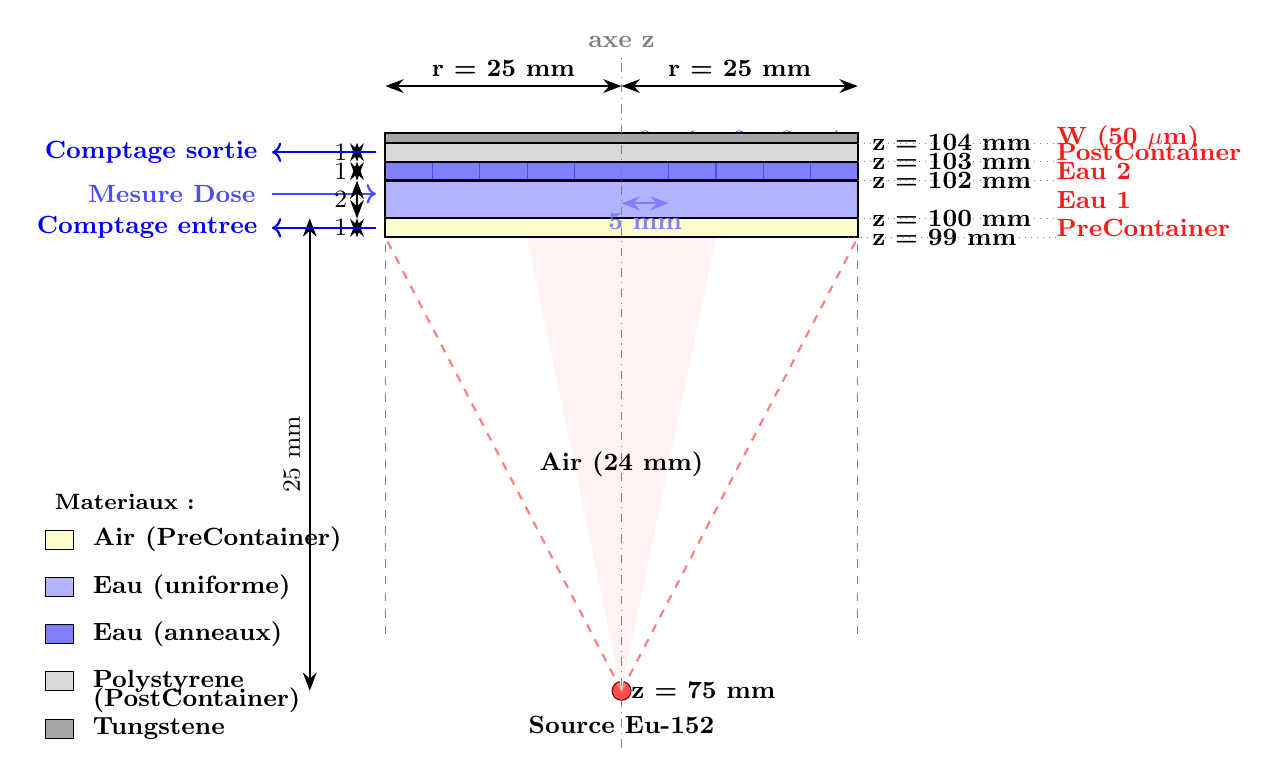
\begin{tikzpicture}[
    scale=0.8,
    x=0.15cm,
    y=0.30cm,
    % Styles
    water/.style={fill=blue!30},
    watertwo/.style={fill=blue!50},
    air/.style={fill=yellow!20},
    polystyrene/.style={fill=gray!30},
    tung/.style={fill=gray!70},
    source/.style={fill=red!70, draw=red!50!black},
    dimension/.style={<->, >=Stealth, thick},
    annot/.style={font=\small},
		annot2/.style={font=\small,red!90}
]

% =============================================================================
% DEFINITION DES COORDONNEES (en mm) - Noms simples
% =============================================================================

\def\rad{25}        % Rayon en mm
\def\srcz{-25}      % Position source
\def\pcbot{-1}      % Bas PreContainer (air)
\def\pctop{0}       % Haut PreContainer = surface eau
\def\wabot{0}       % Bas Eau 1
\def\watop{2}       % Haut Eau 1
\def\wbbot{2}       % Bas Eau 2 (anneaux)
\def\wbtop{3}       % Haut Eau 2
\def\psbot{3}       % Bas Polystyrene
\def\pstop{4}       % Haut Polystyrene
\def\wbot{4}        % Bas Tungstene
\def\wtop{4.5}      % Haut Tungstene

% =============================================================================
% SOURCE Eu-152
% =============================================================================

\fill[source] (0,\srcz) circle (1.5mm);
\node[annot, below=2mm] at (0,\srcz) {\textbf{Source Eu-152}};

% Cone d'emission
\draw[red!50, dashed, thick] (0,\srcz) -- (\rad,\pcbot);
\draw[red!50, dashed, thick] (0,\srcz) -- (-\rad,\pcbot);

% Zone du cone
\fill[red!5] (0,\srcz) -- (10,\pcbot) -- (-10,\pcbot) -- cycle;

% =============================================================================
% AIR (gap source - PreContainer)
% =============================================================================

\draw[gray, thin, dashed] (-\rad,\srcz+3) -- (-\rad,\pcbot);
\draw[gray, thin, dashed] (\rad,\srcz+3) -- (\rad,\pcbot);
\node[annot, black] at (0, -13) {\textbf{Air (24 mm)}};

% =============================================================================
% PRECONTAINER PLANE (Air, 1 mm)
% =============================================================================

\draw[air, thick] (-\rad,\pcbot) rectangle (\rad,\pctop);
\draw[black] (-\rad,\pcbot) rectangle (\rad,\pctop);

\node[annot2, right] at (\rad+20, -0.5) {\textbf{PreContainer}};

% =============================================================================
% EAU 1 (2 mm)
% =============================================================================

\draw[water, thick] (-\rad,\wabot) rectangle (\rad,\watop);
\draw[black] (-\rad,\wabot) rectangle (\rad,\watop);
\node[annot2, right] at (\rad+20, 1) {\textbf{Eau 1}};

% =============================================================================
% EAU 2 (1 mm) - Anneaux
% =============================================================================

\draw[watertwo, thick] (-\rad,\wbbot) rectangle (\rad,\wbtop);

\foreach \r in {5, 10, 15, 20} {
    \draw[blue!70, thin] (-\r,\wbbot) -- (-\r,\wbtop);
    \draw[blue!70, thin] (\r,\wbbot) -- (\r,\wbtop);
}

\draw[black, thick] (-\rad,\wbbot) rectangle (\rad,\wbtop);

% Labels des anneaux
\node[annot, blue!70] at (2.5, 4.2) {0};
\node[annot, blue!70] at (7.5, 4.2) {1};
\node[annot, blue!70] at (12.5, 4.2) {2};
\node[annot, blue!70] at (17.5, 4.2) {3};
\node[annot, blue!70] at (22.5, 4.2) {4};

\node[annot2, right] at (\rad+20, 2.5) {\textbf{Eau 2}};

% Fleche surface eau
\draw[->, thick, blue!70] (-\rad-12, 1.3) -- (-\rad-1, 1.3);
\node[annot, right, blue!70] at (-\rad-12.5-20, 1.3) {\textbf{Mesure Dose}};

% =============================================================================
% POSTCONTAINER = POLYSTYRENE (1 mm)
% =============================================================================

\draw[polystyrene, thick] (-\rad,\psbot) rectangle (\rad,\pstop);
\draw[black] (-\rad,\psbot) rectangle (\rad,\pstop);

\node[annot2, right] at (\rad+20, 3.5) {\textbf{PostContainer}};

% =============================================================================
% TUNGSTENE (50 um)
% =============================================================================

\draw[tung, thick] (-\rad,\wbot) rectangle (\rad,\wtop);
\draw[black] (-\rad,\wbot) rectangle (\rad,\wtop);
\node[annot2, right] at (\rad+20, 4.25) {\textbf{W (50 $\mu$m)}};


% =============================================================================
% COTATIONS
% =============================================================================

% Distance source-eau
\draw[dimension] (-\rad-8, \srcz) -- (-\rad-8, \pctop);
\node[annot, left, rotate=90, anchor=south] at (-\rad-8, -12.5) {25 mm};

% Epaisseurs
\draw[dimension] (-\rad-3, \pcbot) -- (-\rad-3, \pctop);
\node[annot, left] at (-\rad-3, -0.5) {1};

\draw[dimension] (-\rad-3, \wabot) -- (-\rad-3, \watop);
\node[annot, left] at (-\rad-3, 1) {2};

\draw[dimension] (-\rad-3, \wbbot) -- (-\rad-3, \wbtop);
\node[annot, left] at (-\rad-3, 2.5) {1};

\draw[dimension] (-\rad-3, \psbot) -- (-\rad-3, \pstop);
\node[annot, left] at (-\rad-3, 3.5) {1};

% Rayon
\draw[dimension] (0, \wtop+2.5) -- (\rad, \wtop+2.5);
\node[annot, above] at (12.5, \wtop+2.5) {\textbf{r = 25 mm}};
\draw[dimension] (0, \wtop+2.5) -- (-\rad, \wtop+2.5);
\node[annot, above] at (-12.5, \wtop+2.5) {\textbf{r = 25 mm}};

% Axe de symetrie
\draw[gray, dash dot, thin] (0, \srcz-3) -- (0, \wtop+4);
\node[annot, gray, above] at (0, \wtop+4) {\textbf{axe z}};

% Largeur anneau
\draw[dimension, blue!50] (0, \wbbot-1.2) -- (5, \wbbot-1.2);
\node[annot, blue!50, below] at (2.5, \wbbot-1.2) {\textbf{5 mm}};

% =============================================================================
% LEGENDE DES POSITIONS Z
% =============================================================================

\node[annot, anchor=west] at (\rad+0.5, \pcbot) {\textbf{z = 99 mm}};
\node[annot, anchor=west] at (\rad+0.5, \pctop) {\textbf{z = 100 mm}};
\node[annot, anchor=west] at (\rad+0.5, \watop) {\textbf{z = 102 mm}};
\node[annot, anchor=west] at (\rad+0.5, \wbtop) {\textbf{z = 103 mm}};
\node[annot, anchor=west] at (\rad+0.5, \pstop) {\textbf{z = 104 mm}}; %\rad+32-5
\node[annot, anchor=west] at (\rad-25, \srcz) {\textbf{z = 75 mm}};

% Lignes de repere
\draw[gray, dotted, very thin] (\rad-1, \pcbot) -- (\rad+21, \pcbot);
\draw[gray, dotted, very thin] (\rad, \pctop) -- (\rad+21, \pctop);
\draw[gray, dotted, very thin] (\rad, \watop) -- (\rad+21, \watop);
\draw[gray, dotted, very thin] (\rad, \wbtop) -- (\rad+21, \wbtop);
\draw[gray, dotted, very thin] (\rad, \pstop) -- (\rad+21, \pstop);
% =============================================================================
% LEGENDE DES MATERIAUX
% =============================================================================

\begin{scope}[shift={(-\rad-28, -10)}]
    \node[font=\footnotesize\bfseries, anchor=west] at (-8, -5) {\textbf{Materiaux} :};
    
    \draw[air] (0-8, 7.5-15) rectangle (3-8, 8.5-15);
    \draw[black] (0-8, 7.5-15) rectangle (3-8, 8.5-15);
    \node[annot, anchor=west] at (4-8, 8-15) {\textbf{Air (PreContainer)}};
    
    \draw[water] (0-8, 5-15) rectangle (3-8, 6-15);
    \draw[black] (0-8, 5-15) rectangle (3-8, 6-15);
    \node[annot, anchor=west] at (4-8, 5.5-15) {\textbf{Eau (uniforme)}};
    
    \draw[watertwo] (0-8, 2.5-15) rectangle (3-8, 3.5-15);
    \draw[black] (0-8, 2.5-15) rectangle (3-8, 3.5-15);
    \node[annot, anchor=west] at (4-8, 3-15) {\textbf{Eau (anneaux)}};
    
    \draw[polystyrene] (0-8, 0-15) rectangle (3-8, 1-15);
    \draw[black] (0-8, 0-15) rectangle (3-8, 1-15);
    \node[annot, anchor=west] at (4-8, 0.5-15) {\textbf{Polystyrene}};
    \node[annot, anchor=west] at (4-8, -0.5-15) {\textbf{(PostContainer)}};
		
		
    \draw[tung] (0-8, -2.5-15) rectangle (3-8, -1.5-15);
    \draw[black] (0-8, -2.5-15) rectangle (3-8, -1.5-15);
    \node[annot, anchor=west] at (4-8, -2-15) {\textbf{Tungstene}};
\end{scope}

% =============================================================================
% ANNOTATIONS SUPPLEMENTAIRES
% =============================================================================

% Plans de comptage
\draw[<-, thick, blue] (-\rad-12, -0.5) -- (-\rad-1, -0.5);
\node[annot, blue, anchor=east] at (-\rad-12.5, -0.5) {\textbf{Comptage entree}};

\draw[<-, thick, blue] (-\rad-12, 3.5) -- (-\rad-1, 3.5);
\node[annot, blue, anchor=east] at (-\rad-12.5, 3.5) {\textbf{Comptage sortie}};
\end{tikzpicture}
\caption{Coupe longitudinale du dispositif Puits Couronne. La source Eu-152 est positionnée à $z = 75$ mm avec un cône d'émission de 45° (demi-angle). l'eau est séparée en deux tranches: 2mm (\textbf{Eau 1}) et 1mm (\textbf{Eau 2}). Les 5 anneaux d'eau concentriques (nuances de bleu) permettent la mesure de dose radiale.}
\end{figure}


\begin{table}[H]
\centering
\captionsetup{labelformat=empty}
\caption{Position en $\bm{z}$ des différents éléments de la géométrie optimisée.}
\begin{tabular}{l c c c c}
\toprule
\footnotesize \textbf{Volume} &\footnotesize  \textbf{Matériau} &\footnotesize  \textbf{$z_{\min}$ (mm)} &\footnotesize \textbf{$z_{\max}$ (mm)} &\footnotesize  \textbf{Épaisseur (mm)} \\
\midrule
\rowcolor{yellow!25}
\footnotesize PreContainerPlane &\footnotesize Air &\footnotesize 99.0 &\footnotesize 100.0 &\footnotesize  1.0 \\
\midrule
\rowcolor{blue!15}
\footnotesize Eau 1 (uniforme) &\footnotesize Eau &\footnotesize  100.0 &\footnotesize 102.0 &\footnotesize 2.0 \\
\midrule
\rowcolor{blue!25}
\footnotesize Eau 2 (anneaux) &\footnotesize  Eau &\footnotesize  102.0 &\footnotesize 103.0 &\footnotesize  1.0 \\
\rowcolor{blue!25}
\footnotesize \textit{Volume de mesure de dose} &         &        &        &     \\
\midrule
\rowcolor{gray!25}
\footnotesize PostContainerPlane &\footnotesize  Polystyrène &\footnotesize  103.0 &\footnotesize 104.0 &\footnotesize  1.0 \\
\midrule
\rowcolor{green!25}
\footnotesize Feuille de tungstène &\footnotesize  W &\footnotesize  104.0 &\footnotesize 104.05 &\footnotesize  0.05 \\
\bottomrule
\end{tabular}
\end{table}

\clearpage

\medskip
\normalsize
\noindent \color{blue}\textbf{Distances caractéristiques}\color{black}
\footnotesize
\medskip

\begin{center}
\begin{tabular}{|c|c|}
\hline
$z = 104.05$ mm & \textit{Bas feuille W} \\
\hline
\multicolumn{2}{|c|}{Feuille W (50 µm)} \\
\hline
$z = 104.0$ mm & \textit{Haut feuille W / Bas PostContainer} \\
\hline
\multicolumn{2}{|c|}{PostContainer - Polystyrène (1 mm)} \\
\hline
$z = 103.0$ mm & \textit{Haut PostContainer / Haut Eau 2} \\
\hline
\multicolumn{2}{|c|}{Eau 2 (1 mm) - Anneaux - MESURE DOSE} \\
\hline
$z = 102.0$ mm & \textit{Bas Eau 2 / Haut Eau 1} \\
\hline
\multicolumn{2}{|c|}{Eau 1 (2 mm) - Volume uniforme} \\
\hline
$z = 100.0$ mm & \textit{Bas Eau 1 = Surface eau / Haut PreContainer} \\
\hline
\multicolumn{2}{|c|}{PreContainer - Air (1 mm)} \\
\hline
$z = 99.0$ mm & \textit{Bas PreContainer} \\
\hline
\multicolumn{2}{|c|}{Air (24 mm)} \\
\hline
$z = 75.0$ mm & \textit{Source Eu-152} \\
\hline
\end{tabular}
\end{center}

%===============================================================================
\normalsize
\noindent \begin{mdframed}[backgroundcolor=orange!20]
\subsection{\color{blue}\textbf{Analyse du taux d'absorption dans l'eau\\par raie gamma}\color{black}}
\end{mdframed}
\footnotesize
%===============================================================================
\medskip

\medskip
\normalsize
\noindent \color{blue}\textbf{Taux d'absorption par raie gamma}\color{black}
\footnotesize
\medskip

\begin{figure}[H]
\centering
\captionsetup{labelformat=empty}
\includegraphics[scale=0.5]{Figures/absorption_par_raie_Water3mm.png}
\caption{\footnotesize \textit{Taux d'absorption dans l'eau (en \%) pour chacune des 13 raies gamma de l'Eu-152. L'axe Y est en échelle logarithmique pour visualiser les valeurs sur plusieurs ordres de grandeur}}
\end{figure}

\noindent \color{blue}\textbf{Dominance des raies X}\color{black} : Les deux raies X à $\sim$40 keV dominent très largement l'absorption avec des taux de \color{blue}\textbf{2.4\%}\color{black} \; et \color{blue}\textbf{2.3\%}\color{black}. Ces raies représentent plus de \color{blue}\textbf{98\%}\color{black} de l'absorption totale dans l'eau. Le taux d'absorption décroît rapidement avec l'énergie. Les raies au-delà de 300 keV ont des taux d'absorption inférieurs à 0.01\%, ce qui signifie que moins d'un photon sur 10\,000 est absorbé dans les 5 mm d'eau. On observe une légère remontée du taux d'absorption pour la raie à 1408 keV. Ceci pourrait être dû à une \color{blue}\textbf{contribution de la création de paires (seuil à 1022 keV)}\color{black} ou à un effet statistique.\\
    
%===============================================================================
\normalsize
\noindent \begin{mdframed}[backgroundcolor=orange!20]
\subsection{\color{blue}\textbf{Analyse des plans de comptage PreContainer et PostContainer}\color{black}}
\end{mdframed}
\footnotesize
%===============================================================================
\medskip

\medskip
\normalsize
\noindent \color{blue}\textbf{Plan PreContainer -- Particules entrant dans l'eau}\color{black}
\footnotesize
\medskip

\begin{figure}[H]
\centering
\captionsetup{labelformat=empty}
\includegraphics[scale=0.5]{Figures/histos_precontainer_Water3mm.png}
\caption{\footnotesize \textbf{Particules entrant dans le volume d'eau (Precontainer)}}
\end{figure}

\medskip
\normalsize
\noindent \color{blue}\textbf{Photons rétrodiffusés (PostContainer, $\bm{-z}$)}\color{black}
\footnotesize
\medskip

\noindent Cette figure caractérise les photons qui, après avoir traversé partiellement l'eau, sont diffusés vers l'arrière (direction $\bm{-z}$) et repassent par le plan PostContainer.

\begin{figure}[H]
\centering
\captionsetup{labelformat=empty}
\includegraphics[scale=0.5]{Figures/histos_postcontainer_photons_backscatter_Water3mm.png}
\caption{\textit{Photons qui, après avoir traversé partiellement l'eau, sont diffusés vers l'arrière (direction $\bm{-z}$) et repassent par le plan PostContainer}}
\end{figure}

\medskip
\normalsize
\noindent \color{blue}\textbf{Électrons transmis (PostContainer, $\bm{+z}$)}\color{black}
\footnotesize
\medskip

\begin{figure}[H]
\centering
\captionsetup{labelformat=empty}
\includegraphics[scale=0.5]{Figures/histos_postcontainer_electrons_transmis_Water3mm.png}
\caption{\textit{Electrons qui traversent l'eau et sortent dans la direction $\bm{+z}$}}
\end{figure}

\clearpage

\medskip
\normalsize
\noindent \color{blue}\textbf{Électrons rétrodiffusés (PostContainer, $\bm{-z}$)}\color{black}
\footnotesize

\medskip
\begin{figure}[h!]
\centering
\captionsetup{labelformat=empty}
\includegraphics[scale=0.5]{Figures/histos_postcontainer_electrons_backscatter_Water3mm.png}
\caption{\textbf{Electrons qui sont rétrodiffusés depuis les structures après l'eau (feuille de tungstène, container) et retournent vers le volume d'eau}}
\end{figure}

%===============================================================================
\normalsize
\noindent \begin{mdframed}[backgroundcolor=orange!20]
\subsection{\color{blue}\textbf{Analyse Dose Couronnes}\color{black}}
\end{mdframed}
\footnotesize
%===============================================================================
\medskip


\medskip
\normalsize
\noindent \color{blue}\textbf{Spectre gamma entrant dans l'eau}\color{black}
\footnotesize
\medskip


\begin{figure}[H]
\centering
\captionsetup{labelformat=empty}
\includegraphics[scale=0.55]{Figures/spectre_gamma_eau_Water3mm.png}
\captionsetup{labelformat=empty}
\caption{\footnotesize \textit{Spectre en énergie des photons gamma qui pénètrent effectivement dans le volume d'eau après traversée du PMMA}}
\end{figure}

\noindent Cette figure montre le spectre en énergie des photons gamma qui pénètrent effectivement dans le volume d'eau (après traversée du PMMA). Elle permet de quantifier l'atténuation et la modification du spectre entre la source et le milieu de mesure.

\medskip
\normalsize
\noindent \color{blue}\textbf{Distribution de dose par anneau}\color{black}
\footnotesize
\medskip

\begin{figure}[H]
\centering
\captionsetup{labelformat=empty}
\includegraphics[scale=0.6]{Figures/dose_par_anneau_Water3mm.png}
\caption{\footnotesize \textit{Distribution de la dose absorbée (en nGy par événement) pour chacun des 5 anneaux concentriques et pour le total}}
\end{figure}

\noindent Cette figure présente six panneaux montrant la distribution de la dose absorbée (en nGy par événement) pour chacun des 5 anneaux concentriques et pour le total. Les distributions sont présentées en échelle logarithmique. Pour chaque anneau, on observe une distribution caractéristique :

\medskip
\normalsize
\noindent \color{blue}\textbf{Énergie déposée par step}\color{black}
\footnotesize
\medskip

\begin{figure}[H]
\centering
\captionsetup{labelformat=empty}
\includegraphics[scale=0.6]{Figures/edep_par_step_Water3mm.png}
\captionsetup{labelformat=empty}
\caption{\footnotesize \textit{spectres d'énergie déposée par step de simulation pour chaque anneau et pour le total dans l'eau}}
\end{figure}

\noindent Cette figure présente les spectres d'énergie déposée par step de simulation pour chaque anneau et pour le total dans l'eau. L'énergie est exprimée en keV.

\clearpage

\medskip
\normalsize
\noindent \color{blue}\textbf{Spectre des électrons secondaires}\color{black}
\footnotesize
\medskip


\begin{figure}[H]
\centering
\captionsetup{labelformat=empty}
\includegraphics[scale=0.55]{Figures/spectre_electrons_Water3mm.png}
\captionsetup{labelformat=empty}
\caption{\footnotesize \textit{Spectre en énergie (keV) des électrons secondaires créés dans le volume d'eau}}
\end{figure}

\noindent Cette figure montre le spectre en énergie (keV) des électrons secondaires créés dans le volume d'eau par les interactions des photons gamma.

\medskip
\normalsize
\noindent \color{blue}\textbf{Taux d'absorption par raie gamma}\color{black}
\footnotesize
\medskip

\noindent Cette figure présente un histogramme en barres du taux d'absorption (en \%) dans l'eau pour chaque raie gamma de l'Eu-152. L'axe Y est en échelle logarithmique.

\begin{figure}[H]
\centering
\captionsetup{labelformat=empty}
\includegraphics[scale=0.5]{Figures/taux_absorption_eau_Water3mm.png}
\captionsetup{labelformat=empty}
\caption{\footnotesize \textit{Taux d'absorption (en \%) dans l'eau pour chaque raie gamma de l'Eu-152}}
\end{figure}


\begin{figure}[H]
\centering
\captionsetup{labelformat=empty}
\includegraphics[scale=0.5]{Figures/absorption_vs_energie_Water3mm.png}
\captionsetup{labelformat=empty}
\caption{\footnotesize \textit{Taux d'absorption dans l'eau en fonction de l'énergie gamma}}
\end{figure}

\end{document}
